\chapter{Optimization of the floor for dynamic performance}
\label{chap5}
Among the studied 180 floors, only 49 of them (27.2\%) have reached the acceptance criterion that the response factor $R$ should not exceed 8 for office buildings under single person excitation, as shown in figure \ref{fig:m1_f1_fail}. The border differentiating acceptable floors and failed floors is easy to recognize, it is exactly the contour line $R=8$ in figure \ref{fig:m1,f1_R1_contour}. Since 72.7\%  of the floor have failed, improvement measures should be conceived. From the viewpoint of practical applications, however, this failure quotient does not have much meaning. It only means that under the artificial $l,l/d,t_v/t_r$ combinations and given scaling scheme, some of these slabs do not function well enough and the others do. If another scaling scheme is given, e.g. 30\% mass of a solid rectangular floor with the same outer geometry instead of 40\%, some acceptable floors right now will fail as well. So this chapter will not specifically deal with the failed floors, but more generally, how to improve dynamic performances of the rib stiffened vaulted floor.
\begin{figure}[H]
\centering
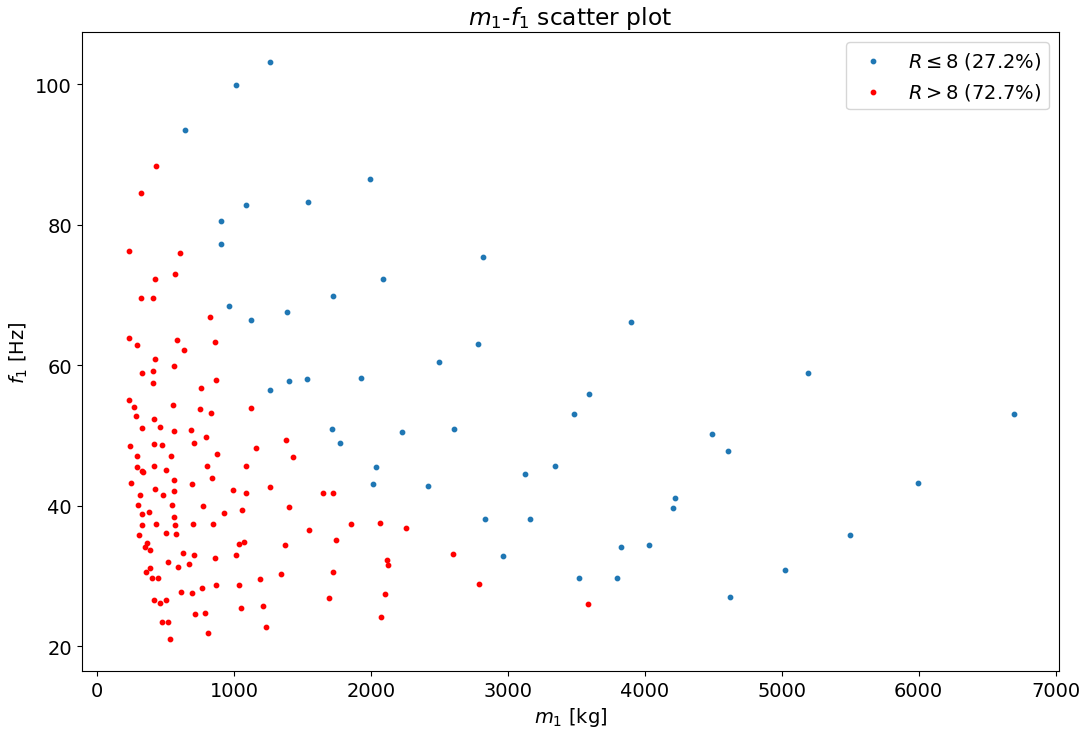
\includegraphics[width=.8\textwidth]{images/m1_f1_fail}
\caption{Acceptable/failed floors shown in $m_1-f_1$ scatter plot}
\label{fig:m1_f1_fail}
\end{figure}

\section{Improvements by mass addition}
Some direct improvement measurements are thinkable just according to the analysis so far. For example, a thicker floor (low $l/d$ value) will lead to a higher natural frequency, more uniformly distributed mass in vault (high $t_v/t_r$ value) can greatly raise the modal mass and slightly increase the natural frequency, the both changes can result in better performances. However, sometimes the $l/d$ ratio cannot be changed as much as it structurally needed, the $t_v/t_r$ ratio cannot go extreme due to production reasons, more refined improvements are necessary. 

The relation between modal response and modal parameters expressed in equation \ref{eqn:R1(m1_f1)} indicates that the raise of product $m_1f_1^{1.5}$ results in a better performance. For an adequately improved floor, for instance if the $t_v/t_r$ ratio has been already raised to a reasonable value, a simultaneous increase in modal mass and natural frequency becomes very difficult. The augment in one value is sometimes only possible at the cost of a reduction in the other. If this trade off can be controlled properly, there will exist space for further improvements. 

The increase in modal mass is easier to conceive and to realize than natural frequency, as the latter is associated with both the stiffness and mass of a structure. Figure \ref{fig:m1,f1_R1_contour} indicates that an increase in modal mass can effectively reduce the response when the modal mass is still low. This finding should apply to floors with 5m span.

The modal mass is computed by
\begin{equation}
\label{eqn:mn_1}
    m_n = \boldsymbol{\phi}_n^T\textbf{m}\boldsymbol{\phi}_n
\end{equation}
it is intuitive that if the mass distribution conforms to the mode shape, the matrix product will generate the highest value. Since the mode shape has its peak in the middle, the mass also should be more concentrated in the middle. One possible way is to keep the existing constant thickness in ribs and vault, and add more mass where appropriate. 

Four factors may influence the effectiveness of improvement: the region where mass is added, the way of adding mass, the amount of mass increase, the geometry of the floor. Two regions have been tried, one is the most inner area (middle 1), the other also includes the second inner ring of panels (middle 2), as shown in figure \ref{fig:middle_1_2}. It is assumed that the additional mass is uniformly distributed on the designated region. Two schemes of adding mass were introduced. One was to change the thickness, which changes the mass and stiff of the panels at the same time. The other scheme is to change the density, which means that only the mass will be altered and the stiffness keeps unchanged. The former simulates the additional mass as the structural component that is monolithically cast and later functions together with the main structure. The latter represents some filling material that solely adds the weight but without any stiffness contribution. The following mass increases in percentage of the original mass were set: [(5),10,(15),20,(25),30]\%. The percentage in brackets are additional mass increments for refinement of the calculation, if certain scheme of adding mass turns out to be better. Only floors of 5m span with following geometric parameters have been evaluated: l/d=[10,15,20], $t_v/t_r=[0.1,1,10]$.

\begin{figure}[H]
\begin{subfigure}[b]{.49\textwidth}
  \centering
  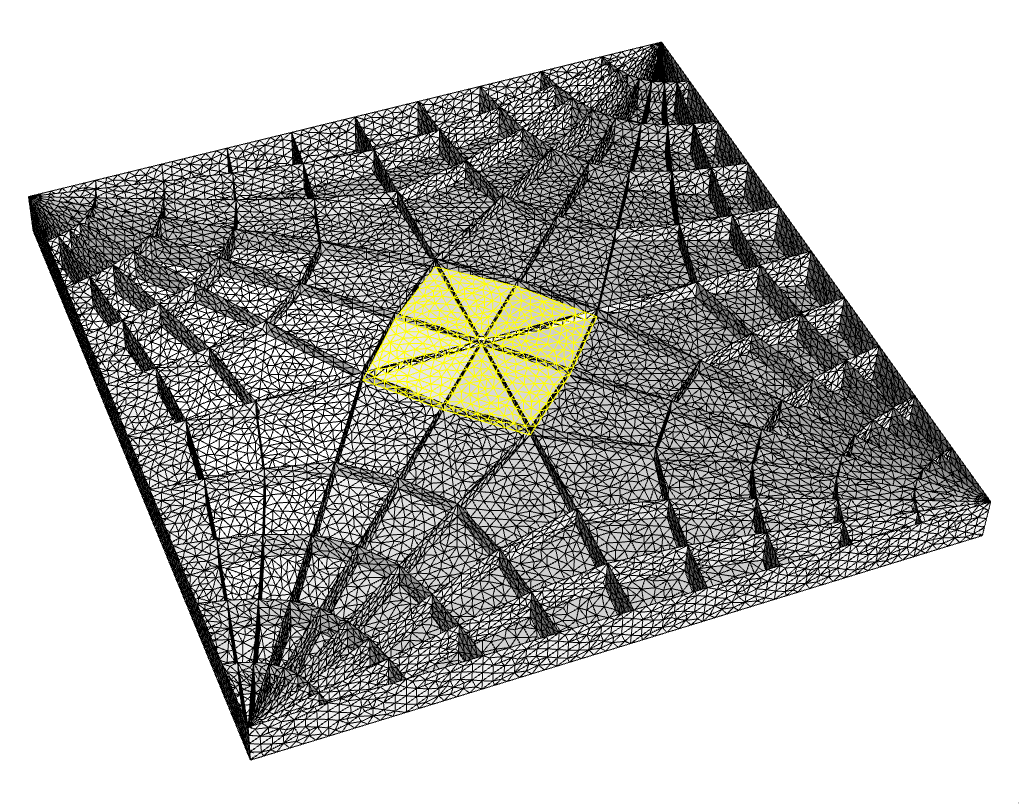
\includegraphics[width=.99\linewidth]{middle_1}
  \caption{Region middle 1}
\end{subfigure}
~
\begin{subfigure}[b]{.49\textwidth}
  \centering
  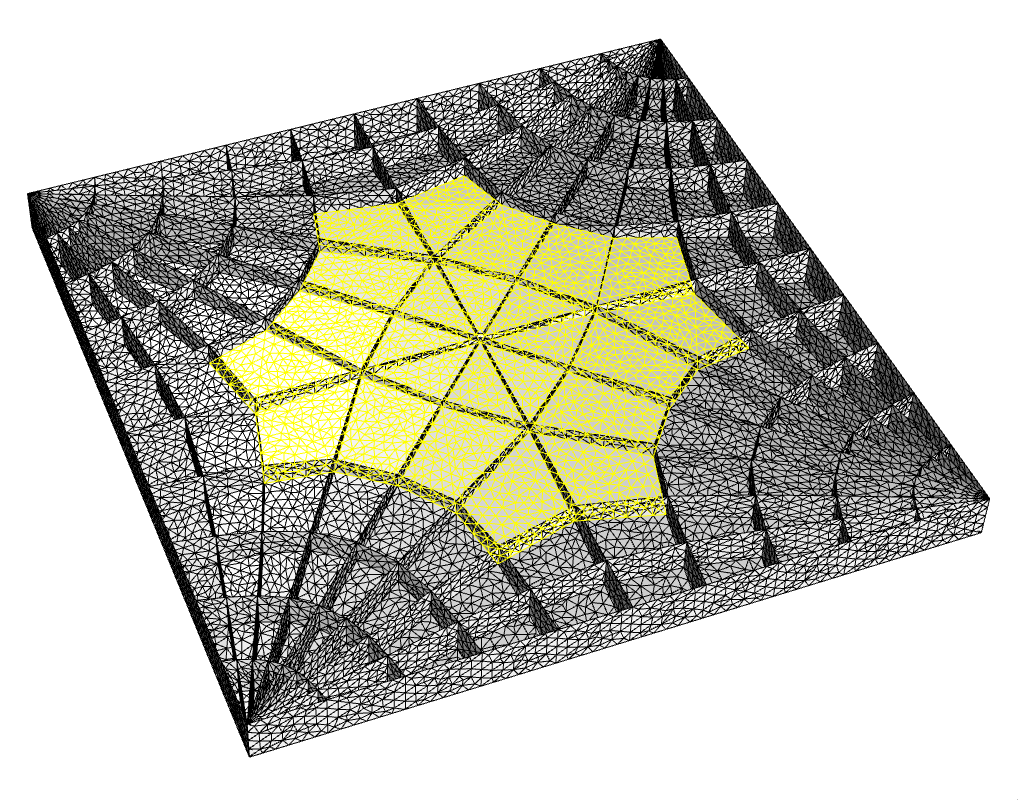
\includegraphics[width=.99\linewidth]{middle_2}
  \caption{Region middle 2}
\end{subfigure}

\caption{Two regions in the middle for additional mass}
\label{fig:middle_1_2}
\end{figure}

Figure \ref{fig:mass_inc_density_middle1} to figure \ref{fig:mass_inc_thickness_middle2} show the normalized (by initial floors) $m_1,f_1,R_1$ of optimized floors with different mass addition schemes and regions in relation to mass increases in percentage. It is evident that mass addition through density change (no stiffness increase) functions not well. The drop in natural frequency compensates much of the increase in modal mass, there appears even some increases in the response for certain combinations. The reduction in natural frequency can be well explained by $\omega_n=\sqrt{k/m}$, when k is unchanged and m increases. Mass addition by thickness change can greatly raise the modal mass, while keeping the drop in natural frequency to a limited degree. Consequently, the improvements are considerable. 
\begin{figure}[H]
\centering
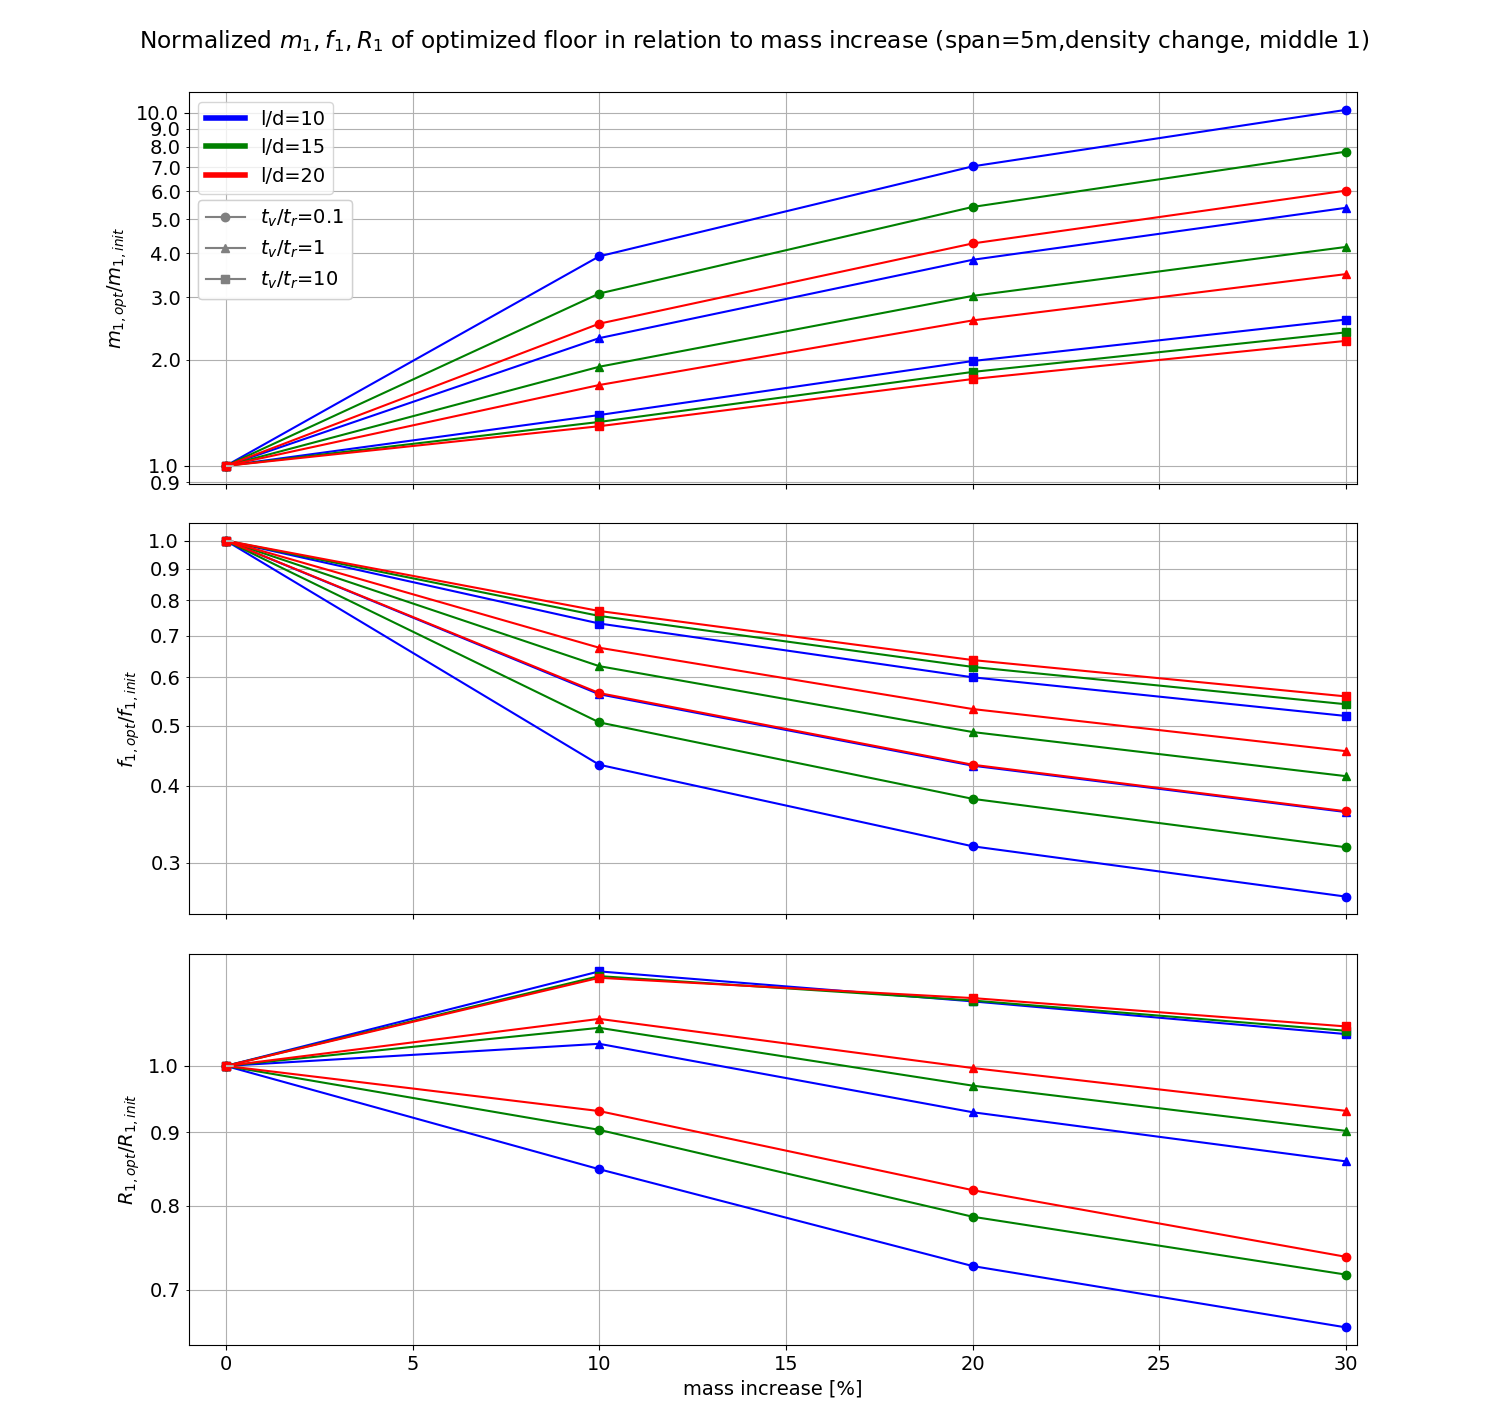
\includegraphics[width=.99\textwidth]{images/mass_inc_density_middle1.png}
\caption{Normalized $m_1,f_1,R_1$ of optimized floor in relation to mass increase (span=5m, density change, middle 1)}
\label{fig:mass_inc_density_middle1}
\end{figure}

\begin{figure}[H]
\centering
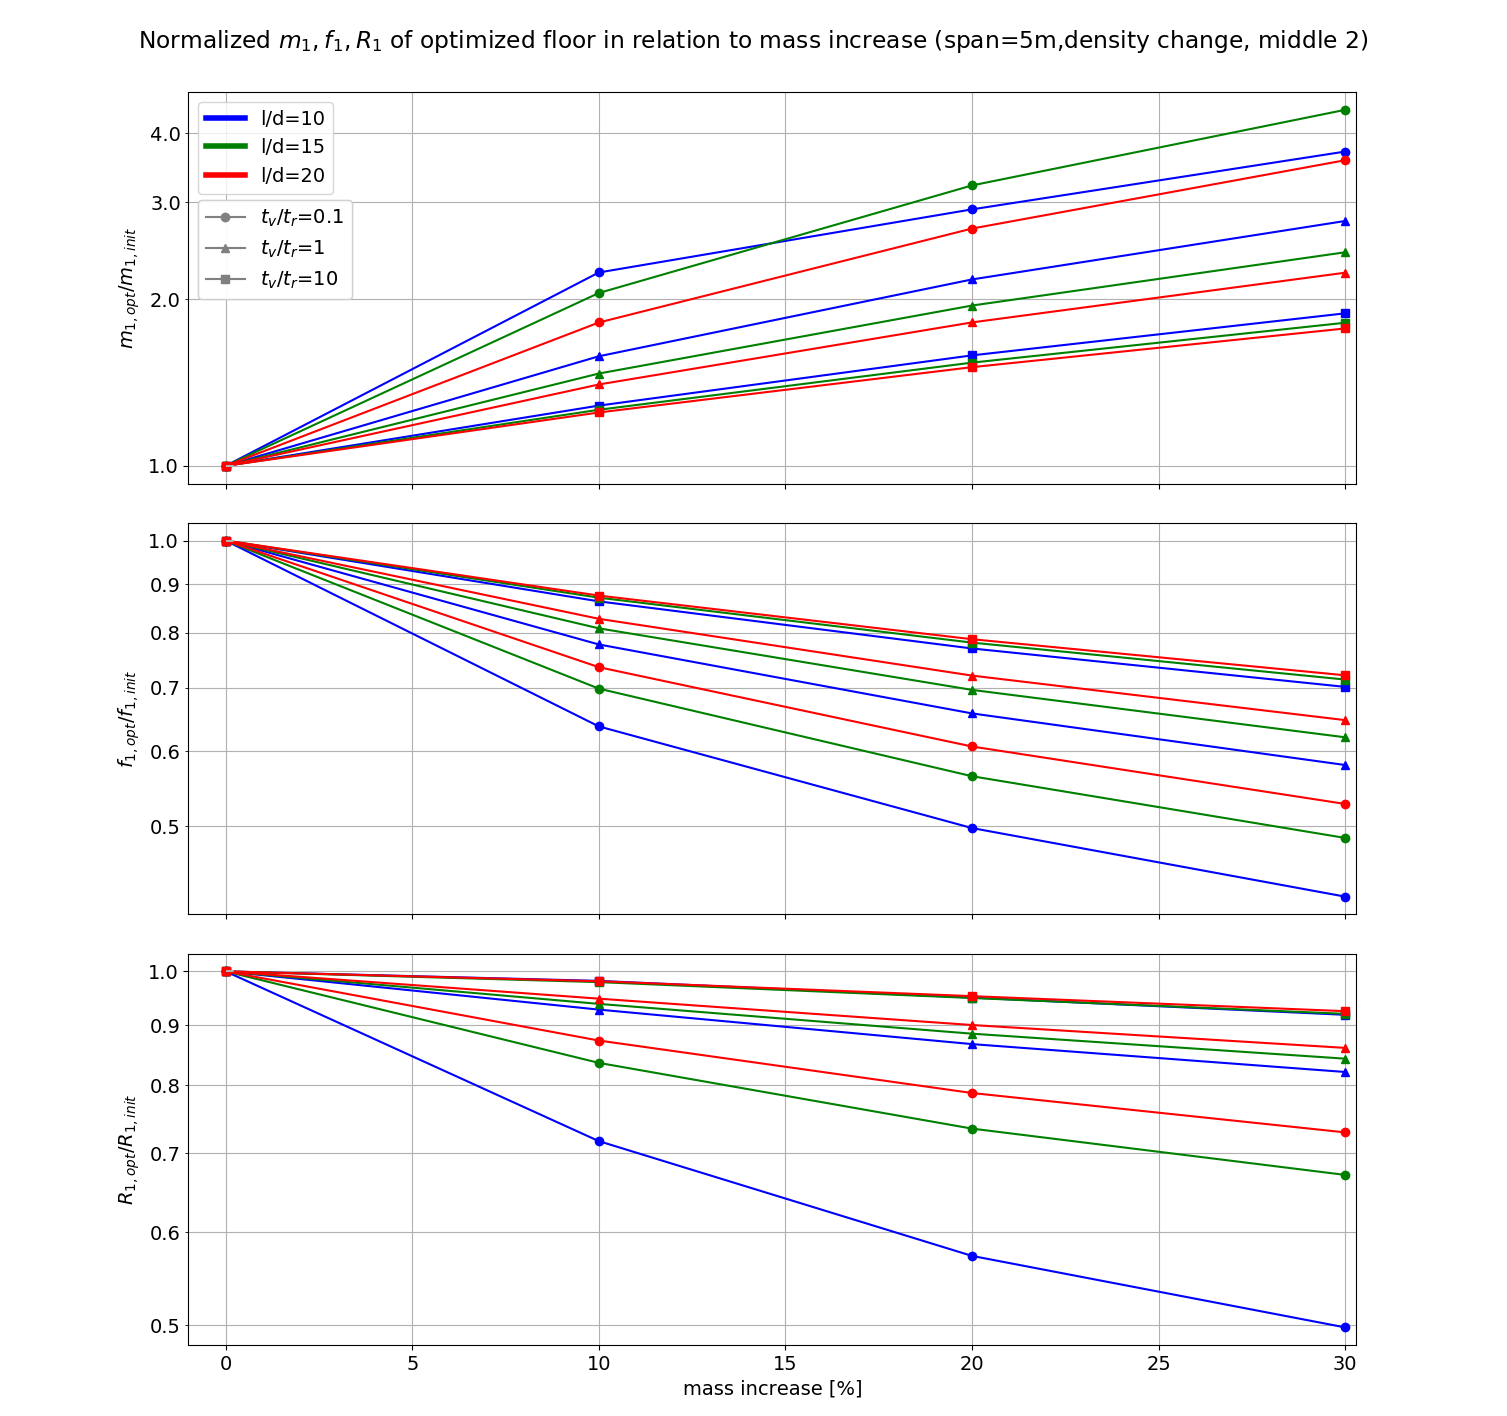
\includegraphics[width=.99\textwidth]{images/mass_inc_density_middle2.png}
\caption{Normalized $m_1,f_1,R_1$ of optimized floor in relation to mass increase (span=5m, density change, middle 2)}
\label{fig:mass_inc_density_middle2}
\end{figure}

\begin{figure}[H]
\centering
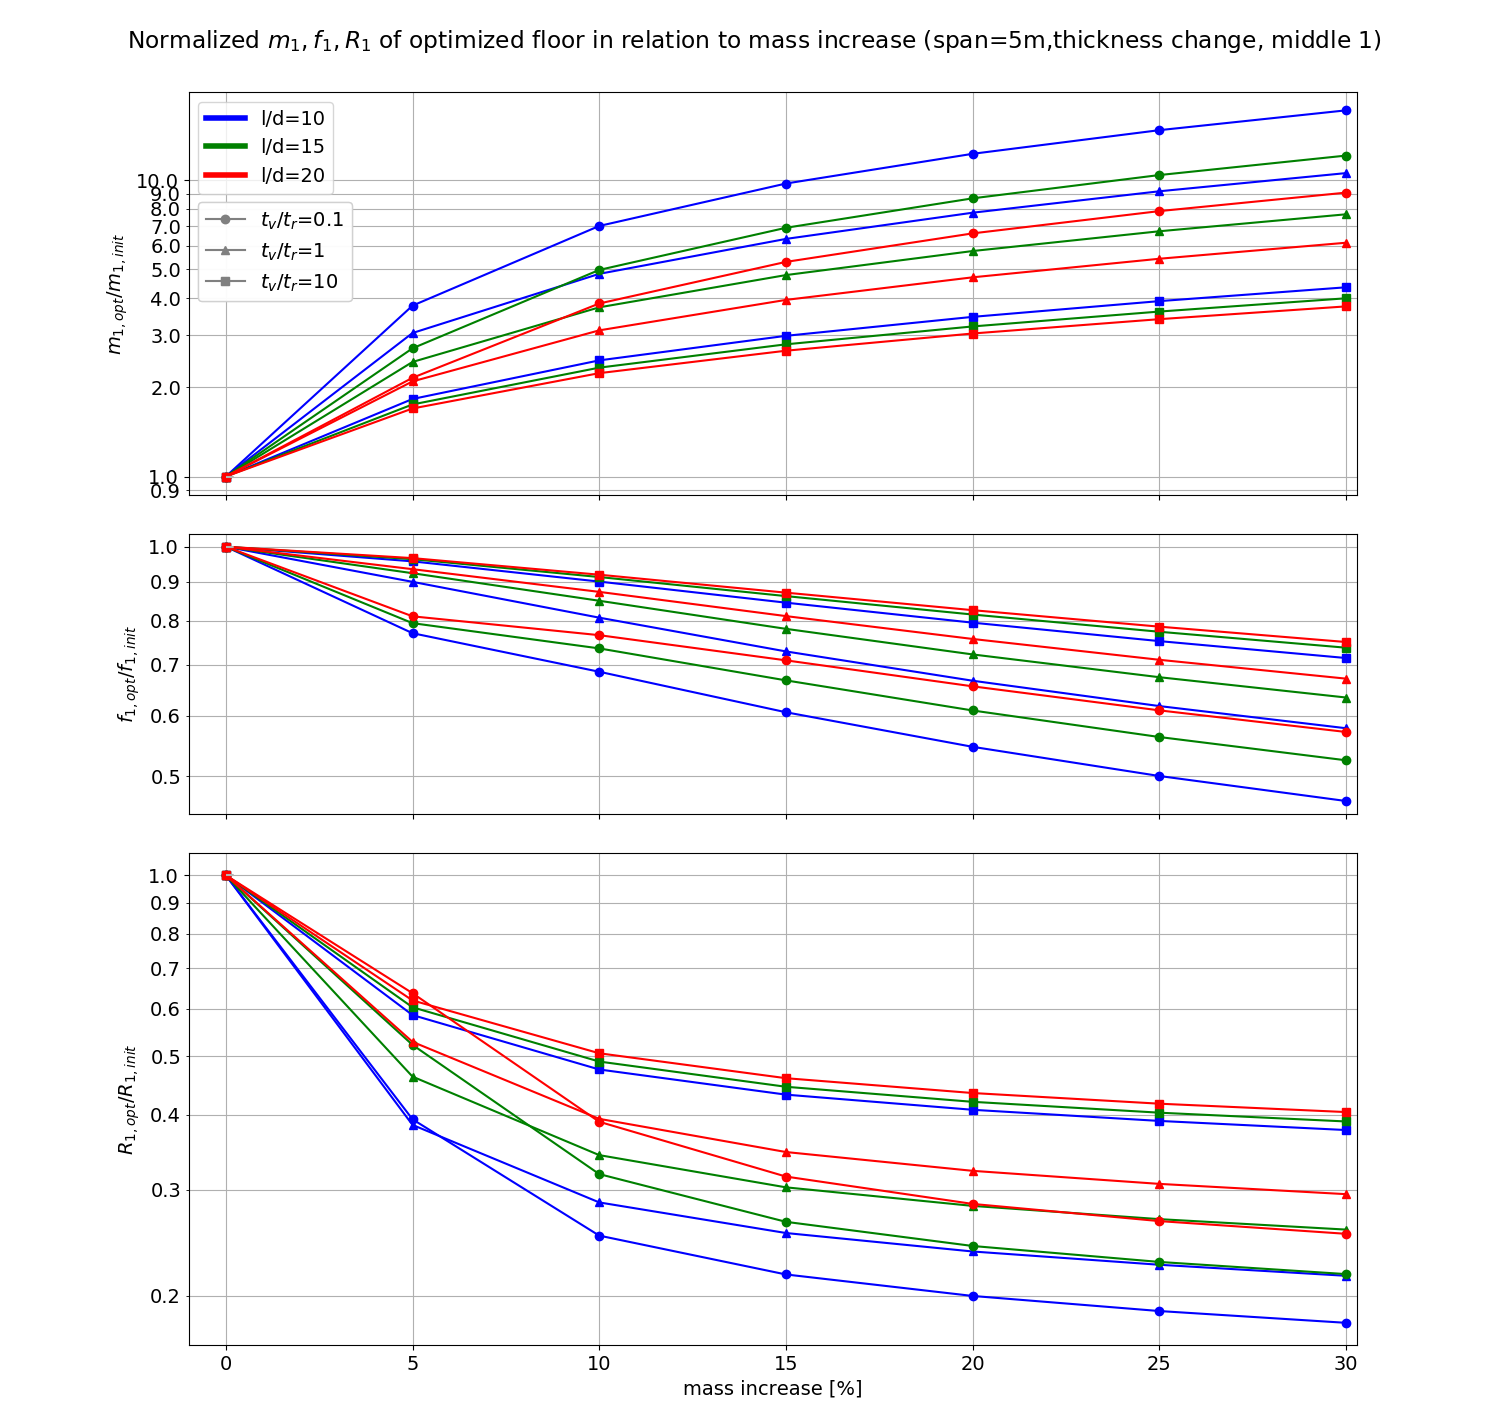
\includegraphics[width=.99\textwidth]{images/mass_inc_thickness_middle1.png}
\caption{Normalized $m_1,f_1,R_1$ of optimized floor in relation to mass increase (span=5m, thickness change, middle 1)}
\label{fig:mass_inc_thickness_middle1}
\end{figure}

\begin{figure}[H]
\centering
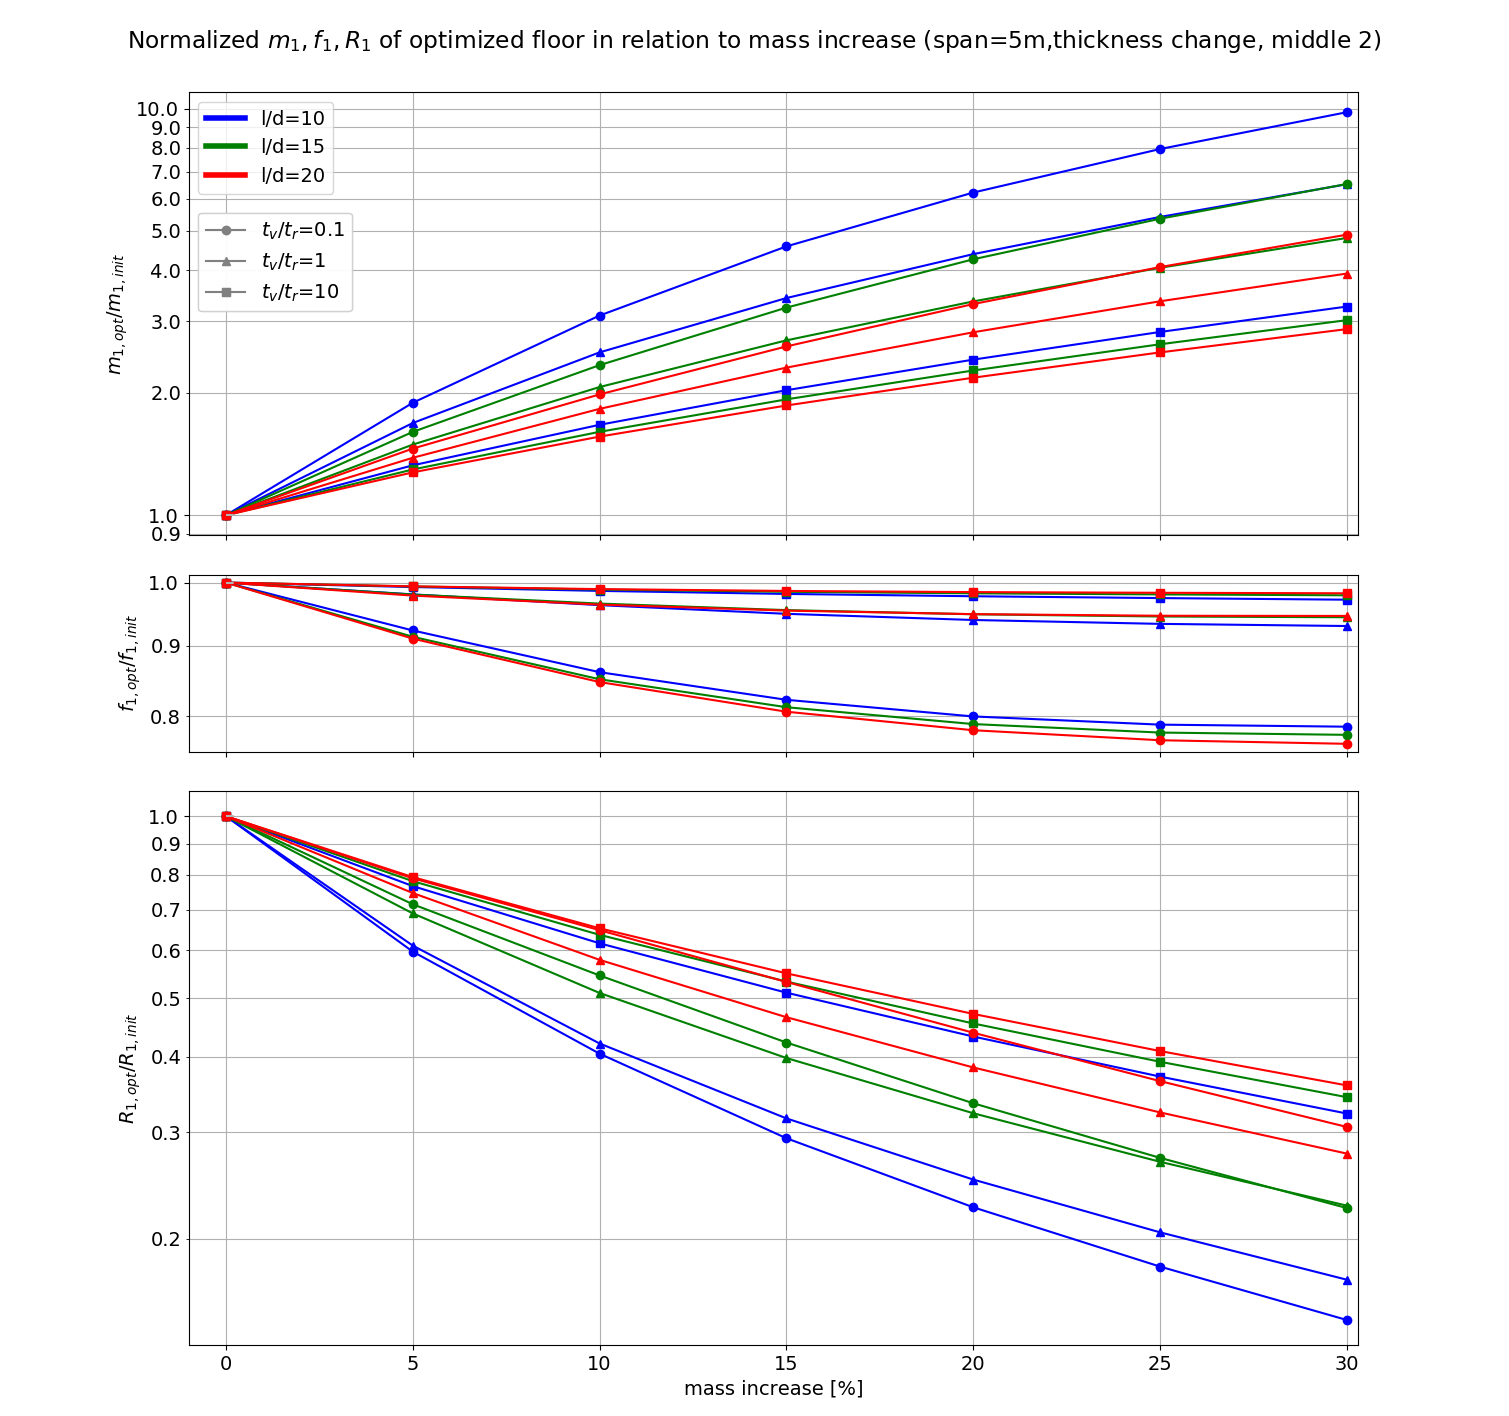
\includegraphics[width=.99\textwidth]{images/mass_inc_thickness_middle2.png}
\caption{Normalized $m_1,f_1,R_1$ of optimized floor in relation to mass increase (span=5m, thickness change, middle 2)}
\label{fig:mass_inc_thickness_middle2}
\end{figure}

The convex shape of the normalized response factor curve indicates reducing performance improvements with raising mass increase percentage. 5\% and 10\% mass increases are most efficient in terms of improvement/mass increase ratio. Table \ref{tab:R1_improv} summaries the effect of mass addition by changing thickness and what that concretely means for the floor\textsuperscript{*} $l=5m, l/d=15, t_v/t_r=1$. The mass addition in region middle 1 seems to generate more response reduction than in middle 2. The defect is the thick vault that may intrude the free space underneath, because the existing vacant space above the vault is not enough for such mass increase. This can also be solved by increasing the height of ribs above the vault. Compared with 5\% mass increase in region middle 1, 10\% mass increase does not bring much improvement. The mass addition in region middle 2 needs less thickness increase to achieve the same mass raise. Although the 5\% mass increase cannot produce a response reduction as high as in middle 1, a higher mass increase can still bring further performance improvement to push the response nearer to the acceptance criterion. In this case, 5\% mass increase in middle 1 and 10\% mass increase in middle 2 are preferred, the final choice depends on other conditions (e.g. if the intrusion in space underneath allowable, if 10\% mass increase is acceptable) and potential further changes (e.g. raise the height of ribs in the middle to create more vacant space for additional structural mass).

{
\renewcommand{\arraystretch}{1.2}
\begin{table}[H]
\caption{Summary of response reduction by mass addition through thickness changing}
\label{tab:R1_improv}
\begin{tabular}{cccccc}
\Xhline{2\arrayrulewidth}
\textbf{region}           & \textbf{mass inc.} & \textbf{resp. red.} & \textbf{\begin{tabular}[c]{@{}c@{}}resp. red.\\ floor\textsuperscript{*}\end{tabular}}   & \textbf{\begin{tabular}[c]{@{}c@{}}thick. inc.\\ floor\textsuperscript{*}\end{tabular}} & \textbf{\begin{tabular}[c]{@{}c@{}}total thick.\\ floor\textsuperscript{*}\end{tabular}} \\ \Xhline{2\arrayrulewidth}
\multirow{2}{*}[-0.8em]{middle 1} & 5\%                    & 36\%-62\%                & \begin{tabular}[c]{@{}c@{}}54\%\\ $R_1: 18.9\xrightarrow{}8.8$\end{tabular}  & 0.106 m                                                                     & 0.163 m                                                                  \\ \cline{2-6}
                          & 10\%                   & 49\%-75\%                & \begin{tabular}[c]{@{}c@{}}66\%\\ $R_1: 18.9\xrightarrow{}6.5$\end{tabular}  & 0.212 m                                                                     & 0.269 m                                                                  \\ \hline
\multirow{2}{*}[-0.8em]{middle 2} & 5\%                    & 20\%-40\%                & \begin{tabular}[c]{@{}c@{}}31\%\\ $R_1: 18.9\xrightarrow{}13.1$\end{tabular} & 0.026 m                                                                     & 0.083 m                                                                  \\ \cline{2-6}
                          & 10\%                   & 35\%-60\%                & \begin{tabular}[c]{@{}c@{}}49\%\\ $R_1: 18.9\xrightarrow{}9.7$\end{tabular}  & 0.052 m                                                                     & 0.109 m                                                                  \\ \Xhline{2\arrayrulewidth}
\end{tabular}
\end{table}
}

These improvements can be illustrated in the $m_1,f_1-R_1$ contour plot \ref{fig:m1_f1_improve}. None of the four schemes are along the most efficient direction - the gradient of $m_1,f_1-R_1$ surface, namely the normal direction of contour lines. Sometimes, designated changes in modal parameters are difficult to realize in reality, as they are tightly correlated.

\begin{figure}[H]
\centering
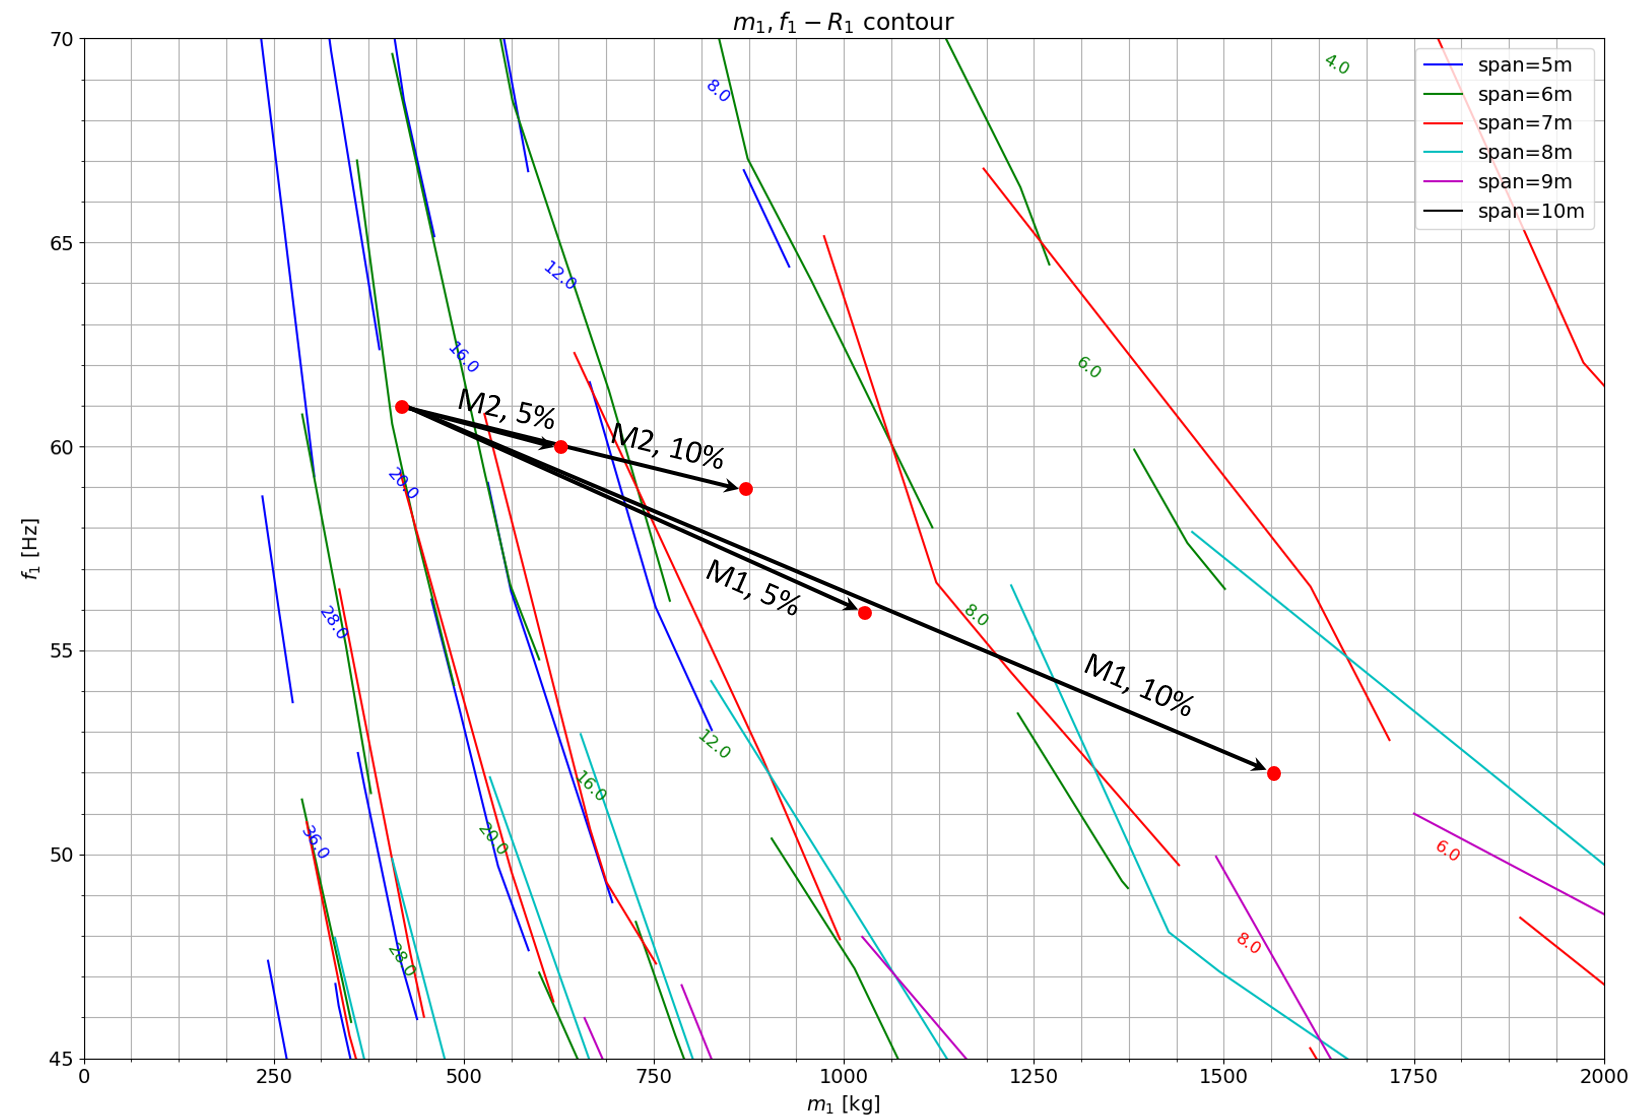
\includegraphics[width=.95\textwidth]{images/m1_f1_improve}
\caption{Four improvement schemes presented on $m_1,f_1-R_1$ contour plot}
\label{fig:m1_f1_improve}
\end{figure}

\section{Surrogate model based optimization}
The research so far, even the improvements by mass addition, is based on the models with uniform thickness in ribs and vault. It is intuitive that a "perfectly" improved floor under constant mass will not have constant thickness everywhere in vault, so will not in ribs. 

\subsection{One-quarter mesh model}
To optimize the floor in a further step, the dimension of the model has to be raised. The dimension of a model represents its complexity, and also the degree of refinement. When $l,l/d$ are kept constant, the previous model has only two dimensions, the thickness of the vault and ribs. To refine the floor, the panels were assigned to 41 groups, each group could have a different thickness. To reduce the computational cost, only one quarter of the slab was modeled, as shown in figure \ref{fig:panels_modelling} (each group is given a different color). There are two boundary surfaces, they are named by their normal directions. To capture the mode shapes that are symmetric about both x and y axis, including the 1st mode, the DOFs on boundary surface x should not move along x axis, and the rotation around y axis should be fixed. For boundary surface y, movement along y and rotation around x should be constrained. The movement and rotation in other directions are free. In addition, the stiffness and mass of the boundary surfaces should be halved, as they are shared by neighboring quarters. Because the main stiffness of the boundary surfaces is in vertical direction, the halving can be roughly achieved by halving the thickness, although it creates inaccuracy in horizontal stiffness. Natural frequencies and modal masses of the one quarter model match well with the symmetric modes of the full model.
\begin{figure}[H]
\centering
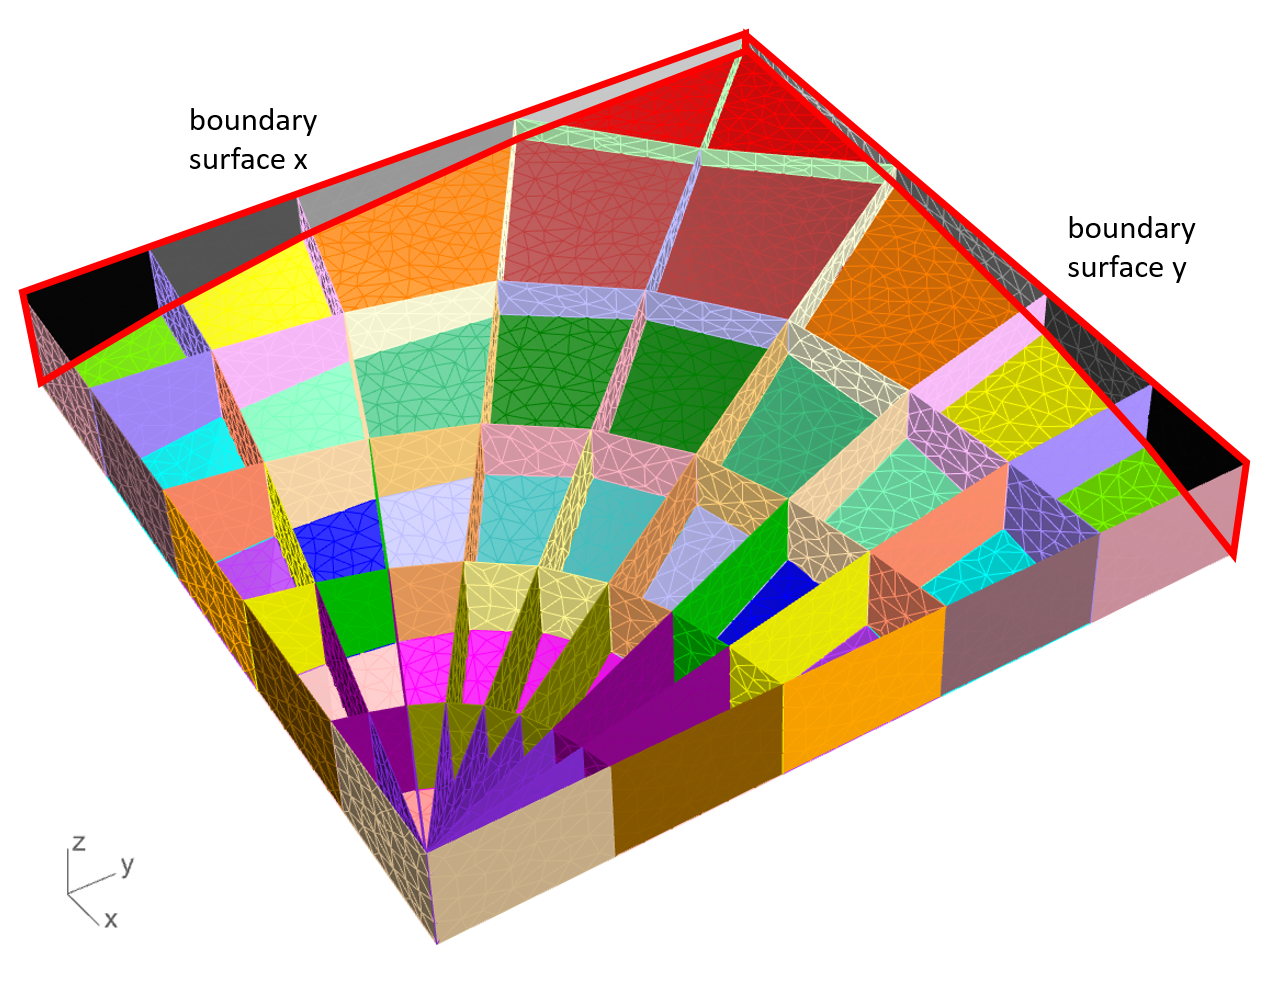
\includegraphics[width=.9\textwidth]{images/panels_modelling}
\caption{One-quarter model of the floor with $l=5m,l/d=15$}
\label{fig:panels_modelling}
\end{figure}

\subsection{Work flow}
For such a complex model with 41 dimensions, manual optimization is impossible. Because the final response cannot be expressed in a closed form of geometric parameters (the thicknesses of the 41 group of panels), no matter implicit or explicit, and the number of dimensions is large, traditional derivative based algorithm is not a good option. One possible solution is the genetic algorithm, which is robust even when there are multiple local optima, the objective function is not smooth and the number of parameters is large. However, even though the GA can accelerate the convergence by selecting "good seeds" and filtering out bad ones, it still requires a large amount of runs of the model. Assume that the model has a population of 100, and needs 200 generations to get converged (already optimistic assumption), then 20000 runs are needed. If one evaluation of such a model needs 1 min, then one optimization process will take two weeks, which is hardly affordable. One possible way to address the optimize problem is to use a surrogate model, which can reflect the essence of the real model to a certain degree but takes muss less time to run.

The concept of optimization through a surrogate model is shown in figure \ref{fig:opt_flowchart}. This is a machine learning alike idea, the accuracy of the final results cannot be guaranteed. They depends on the input sampling, the complexity of the model, the amount of real data and the form of surrogate model, etc. To "train" the surrogate model, certain evaluations of the full model, namely experimental designs, are necessary. Using the real (geometric input, response factor output) data sets, parameters in the surrogate model can be determined. The GA optimization will be no longer applied on the full model, but the surrogate model that skips the intermediate steps and directly maps the geometric input to the response factor output. Once the optimization is finished, the input of the optimized surrogate model will be used to recalculate the authentic response factor. Because the optimized input is sometimes not within the input samples that were used to train the surrogate model, the prediction from it can be biased. They values predicted by the surrogate model usually show the trend, but not necessarily the exact numbers. 

\begin{figure}[H]
\centering
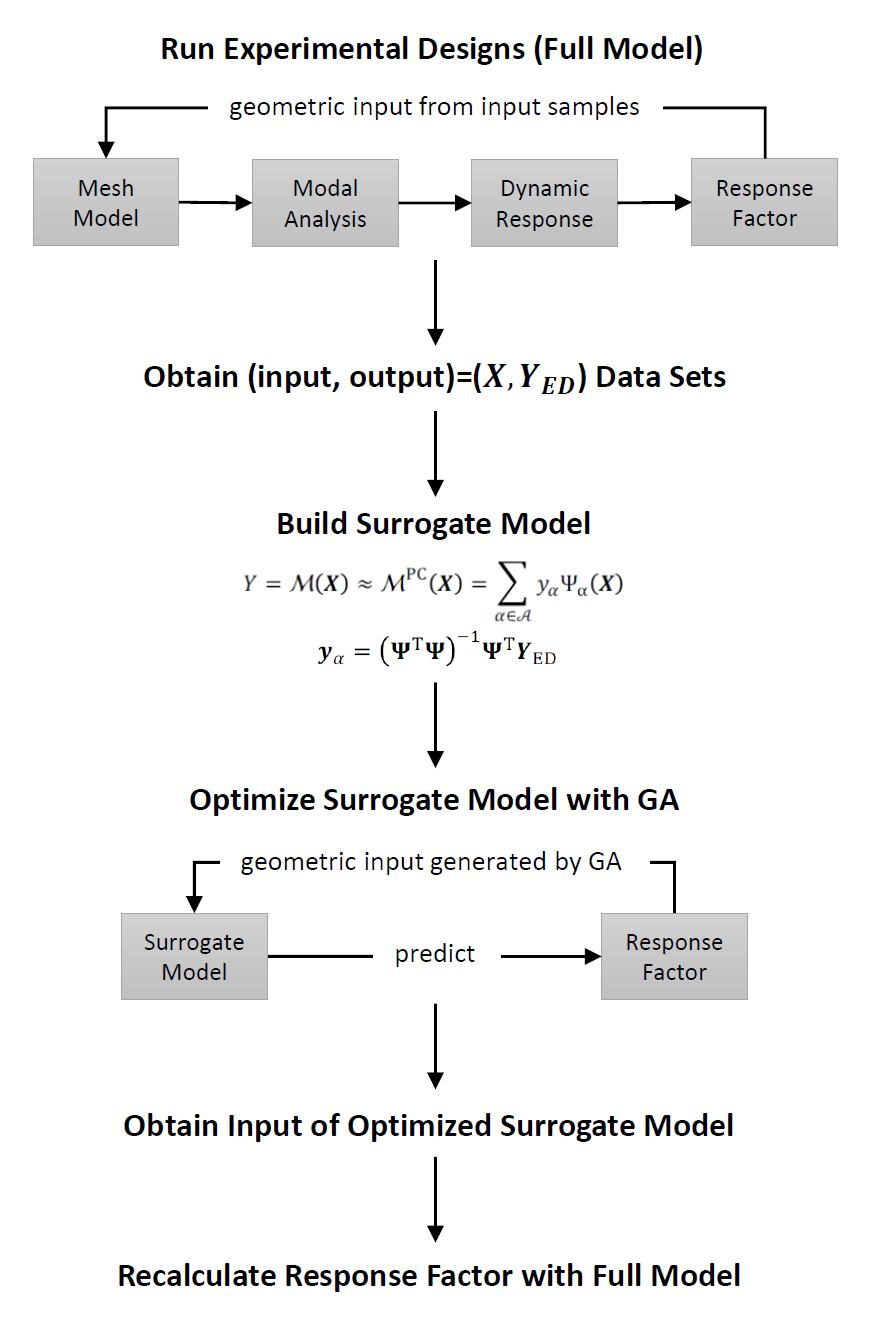
\includegraphics[width=.7\textwidth]{images/opt_flowchart}
\caption{Flow chart of surrogate model based optimization}
\label{fig:opt_flowchart}
\end{figure}

\subsection{PCE surrogate model}
The are several ways to build the surrogate model, PCE (polynomial chaos expansion), Kriging model, neural nets, etc. Subject to the limitation of the author's knowledge and time frame for the master's thesis, only the PCE model has been implemented. It does not mean that it is the best option.

PCE is usually applied in a stochastic process to solve uncertainty propagation problems. It can depict the uncertainty in the output resulted from the uncertainty in the input accurately  enough based on a limited number of experimental designs. The problem that PCE addresses has similarities and also difference with the present problem of the floors. They both have a certain bandwidth in which the input can vary, and both have only limited number of evaluations of the full model. The difference is that, the distribution (uncertainty) of the output is not a concern in this optimization problem, therefore some modifications of the classical PCE can be made.

To approximate the real model $\mathcal{M}(\boldsymbol{X}$), a surrogate truncated PCE model can be built
\begin{equation}
    Y=\mathcal{M}(\boldsymbol{X})\approx \mathcal{M}^{PC}(\boldsymbol{X})=\sum_{\alpha\in \mathcal{A}}y_{\alpha}\Psi_{\alpha}(\boldsymbol{X})
\end{equation}
\noindent
The task is then to develop a set of appropriate polynomial basis $\Psi_{\alpha}$ and search for corresponding coefficients $y_{\alpha}$. For the classic PCE, the multivariate polynomial bases are orthogonal to each other and they are deduced with recurrence relations. In that way, the statistical characteristics (mean and standard deviation) of the model can be easily obtained by evaluating the coefficients. But the statistical characteristics is not of interest to the present problem, and the evaluation of orthogonal polynomial bases is much more time consuming than free bases (about three times more time based on the author's codes), the latter would be chosen to build the polynomial.

For a model with dimension $M$, the total degree of polynomial $p$, over-sampling rate $k$, the multi-indices $\boldsymbol{\alpha}$ can be defined
\begin{equation}
    \boldsymbol{\alpha}=\{\alpha_1,...,\alpha_M\}, \text{ of degree }|\boldsymbol{\alpha}|=\sum_{i=1}^M \alpha_i  
\end{equation}
\noindent
The associated multivariate polynomial reads
\begin{equation}
    \Psi_{\boldsymbol{\alpha}}(\boldsymbol{x})=\prod_{i=1}^M\Psi_{\alpha_i}^{(i)}(x_i)
\end{equation}
\noindent
where $\Psi_{\alpha_i}^{(i)}(x_i)$ is the univariate polynomial of degree $\alpha_i$ in form
\begin{equation}
    \Psi_{\alpha_i}^{(i)}(x_i)=x_i^{\alpha_i}
\end{equation}
\noindent
The set of all possible multi-indices $\boldsymbol{\alpha}$
\begin{equation}
    \mathcal{A}^{M,p}=\{\alpha\in\mathbb{N}^M : |\alpha|\leq p\}
\end{equation}
its cardinality, also the number of coefficients
\begin{equation}
    P=\text{card }\mathcal{A}^{M,p}=\begin{pmatrix} M+p\\p\end{pmatrix}=\frac{(M+p)!}{M!p!}
\end{equation}
The number of evaluations of the full model for experimental designs
\begin{equation}
    n=kP
\end{equation}
When the input $\boldsymbol{X}_{ED}$ and output $\boldsymbol{Y}_{ED}$ are available, the polynomial coefficients can be obtained via least-square minimization 
\begin{equation}
    \boldsymbol{y}_{\alpha}=(\boldsymbol{\Psi}^T\boldsymbol{\Psi})^{-1}\boldsymbol{\Psi}^T\boldsymbol{Y}_{ED}
\end{equation}
\noindent
where $\boldsymbol{\Psi}$ matrix is assembled by
\begin{equation}
\label{eqn:Psi}
    \boldsymbol{\Psi}=\Psi_{ij}(\boldsymbol{X}_{ED})=\Psi_j(\boldsymbol{X}_{ED}^{(i)})=
    \begin{pmatrix}
    \Psi_1(x^{(1)})&\cdots&\Psi_P(x^{(1)})\\
    \vdots         &\ddots&\vdots\\
    \Psi_1(x^{(n)})&\cdots&\Psi_P(x^{(n)})
    \end{pmatrix}
\end{equation}
\noindent
When the PCE is built, meaning that the coefficients are already known, predictions can be made by
\begin{equation}
    \boldsymbol{Y}_{\text{pred}}=\mathcal{M}^{PC}(\boldsymbol{X})=\sum_{\alpha\in\mathcal{A}}y_{\alpha}\Psi_{\alpha}(\boldsymbol{X})=\boldsymbol{\Psi}\boldsymbol{y}_{\alpha}
\end{equation}
where $\boldsymbol{X}$ is the actual thickness sets whose responses are to be predicted.

For the model with dimensions $M=41$, only the first degree polynomial is used and an over-sampling rate $k=2$ to avoid over-fitting, the full model needs to be evaluated $n=84$ times, which is easily affordable. When the second degree polynomial and the same over-sampling rate are adopted, $n=1806$, which will take 30 hours to run. The necessary number of evaluations raises exponentially with the dimension of the model and the maximal degree of polynomial. 

\subsection{Input sampling}
Due to the time restriction, only the PCE models with the first degree polynomial have been built. One is for the floor $l=5m, l/d=10$, with nonuniform input samples for the experimental designs, the other is for the floor $l=5m, l/d=15$, with uniform input samples. The sampling of bot floors is shown in figure \ref{fig:sample}. 
\begin{figure}[H]
\begin{subfigure}[b]{.49\textwidth}
  \centering
  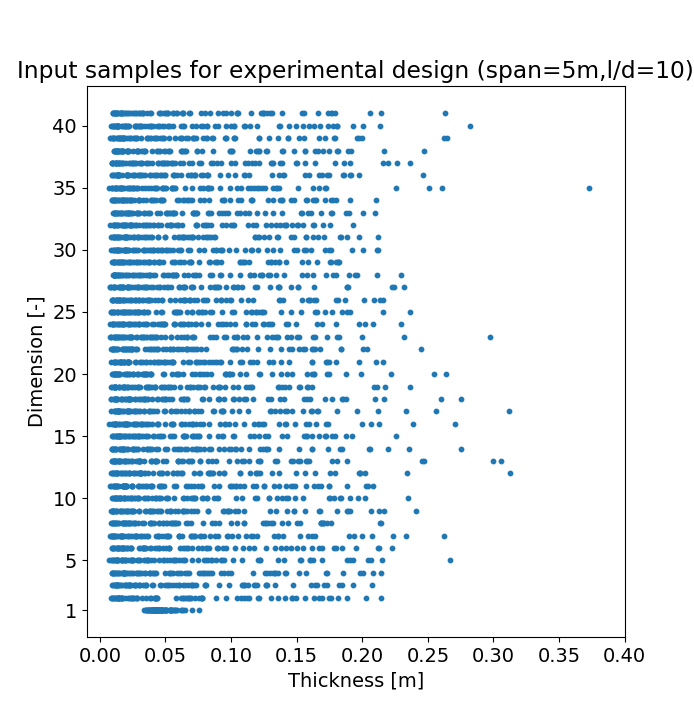
\includegraphics[width=.99\linewidth]{images/sample_10.png}
  \caption{$l=5m,l/d=10$}
\end{subfigure}
~
\begin{subfigure}[b]{.49\textwidth}
  \centering
  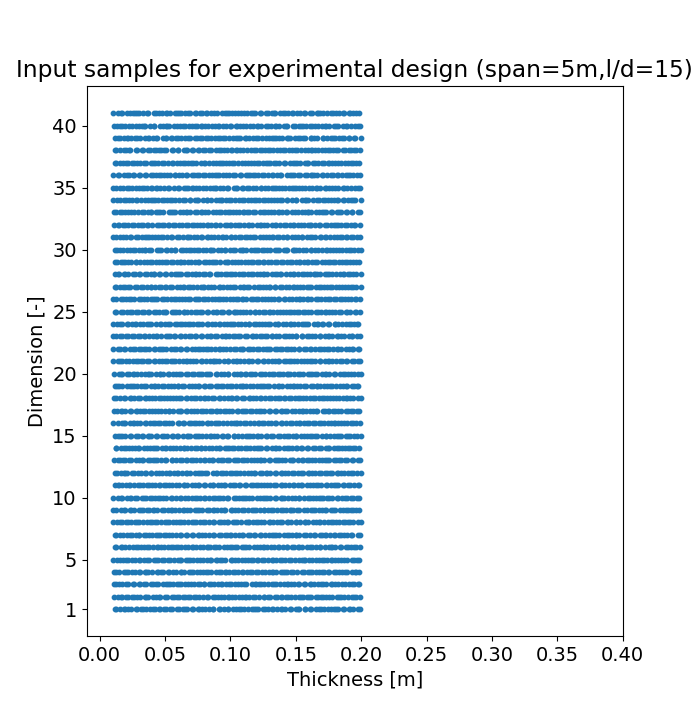
\includegraphics[width=.99\linewidth]{images/sample_15.png}
  \caption{$l=5m,/d=15$}
\end{subfigure}

\caption{Thickness input samples of two floors}
\label{fig:sample}
\end{figure}

In the first floor, the sampling is probably not smart enough. The idea was, since the actual thicknesses cannot be really random (because the total mass of the floor is constant), then one dimension can be chosen as the basis, the ratios of other dimensions to this dimension can be random (ranging from 1/5 to 5). What really maters is the ratios, as concrete numbers will be calculated based on the constant mass. The plot (a) in figure \ref{fig:sample} shows the scaled thickness with the first dimension as the basis. It can be seen that the range of the first dimension is much narrower than other dimensions, and the greater the thickness, the less sample points there are. For the second floor, a pure uniform distribution (Latin Hypercube Sampling for more evenly distributed sampling) between [0.01,0.2]m is adopted. Since the input samples are for the experimental designs, and the goal is to train the surrogate model instead of calculating the response in reality, there is no need to sample the points as they may actually occur under the constraint of constant mass.

\subsection{Results of GA optimization}
The thickness ratio between thickest panel and the thinnest can be given in the GA as the upper bound, while the lower bound is always set to be 1. Figure \ref{fig:opt_floor_l2d10} and \ref{fig:opt_floor_l2d15} show the optimized mass distribution with different maximal thickness ratios for floor $l=5m,l/d=10$ and $l=5m,l/d=15$ respectively. The darker the color, the thicker the panels. It is evident that the optimized figure depends on the allowable thickness ratio. The higher this value, the more freedom the mass has to concentrate on where minimizing the response. Observe that for any allowable thickness ratio, there exist only extreme thicknesses after optimization. This may be due to the limitation of this PCE model. As only the first degree polynomial was used, it could not form any bowl alike local optimum, the optimum is always obtained on boundaries. However, it is possible that the ideally fully optimized models also do not have intermediate thickness values. 

\begin{figure}[H]
\begin{subfigure}[b]{.32\textwidth}
  \centering
  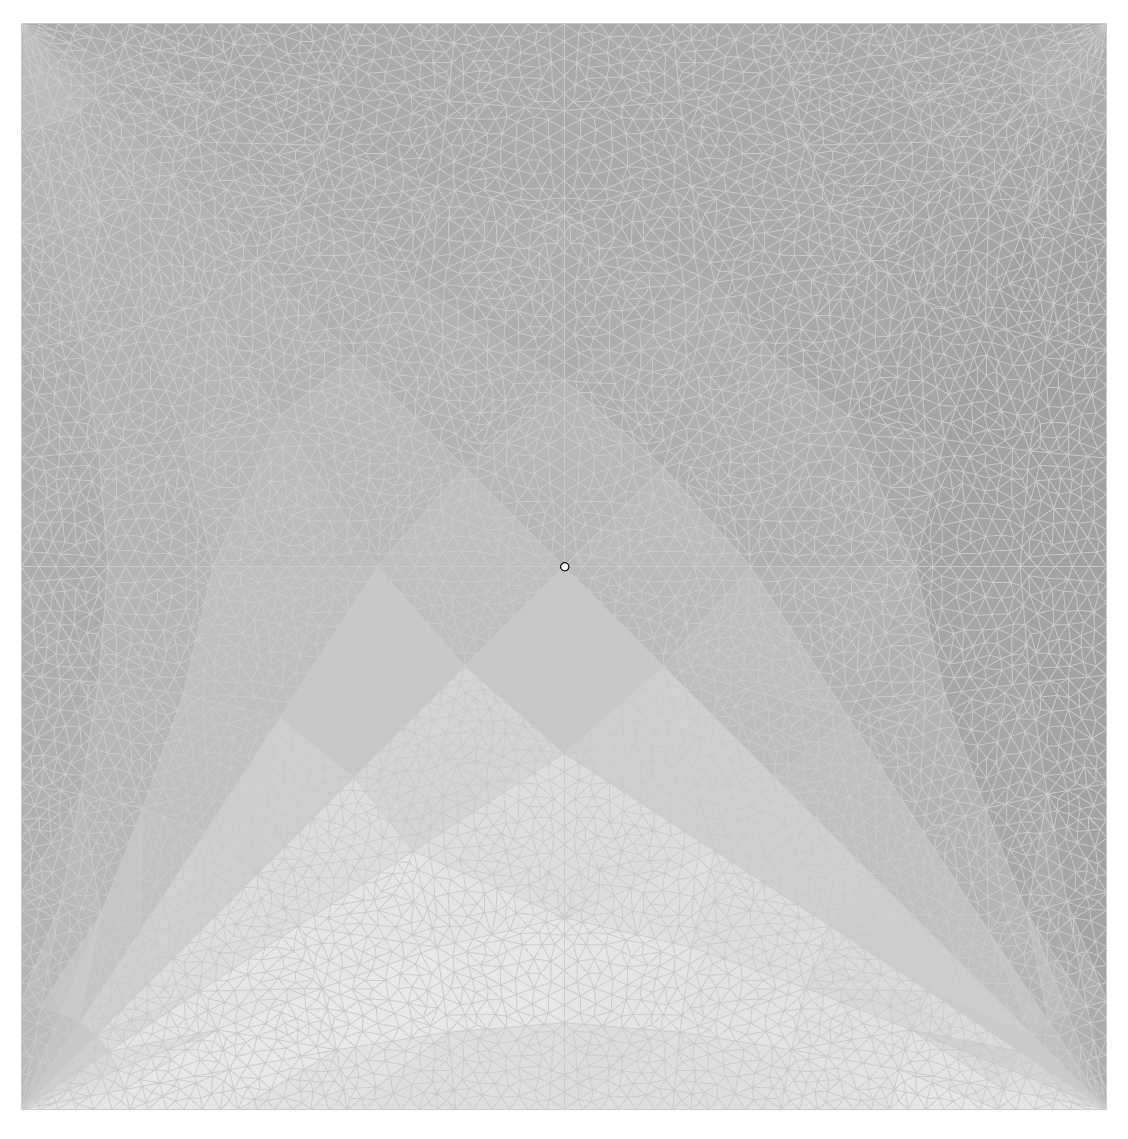
\includegraphics[width=.99\linewidth]{images/t_opt_l2d10_gamma1}
  \caption{$t_{max}/t_{min}=1$}
\end{subfigure}
~
\begin{subfigure}[b]{.32\textwidth}
  \centering
  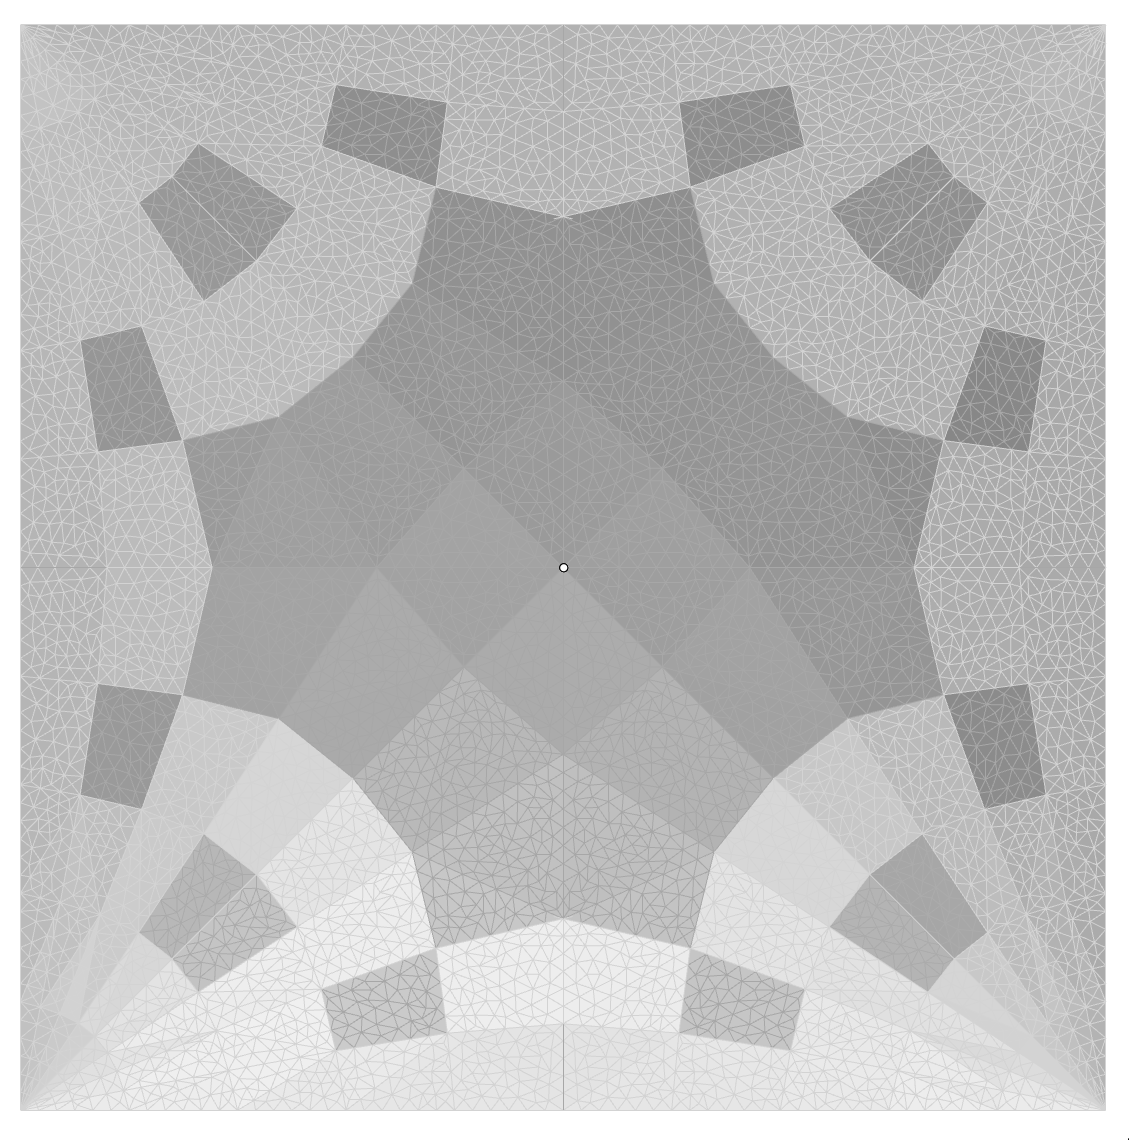
\includegraphics[width=.99\linewidth]{images/t_opt_l2d10_gamma2}
  \caption{$t_{max}/t_{min}=2$}
\end{subfigure}
~
\begin{subfigure}[b]{.32\textwidth}
  \centering
  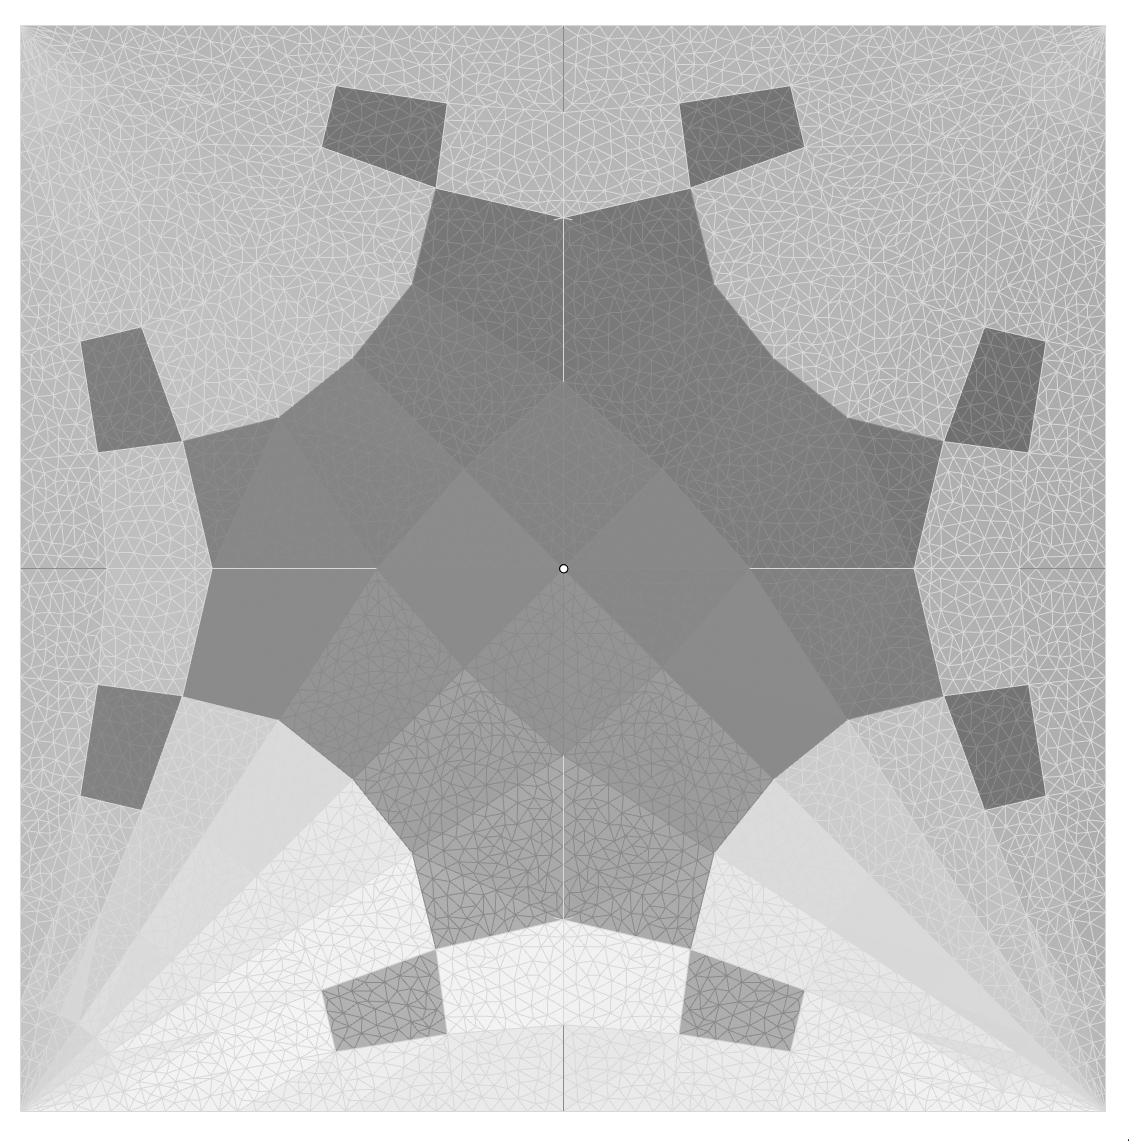
\includegraphics[width=.99\linewidth]{images/t_opt_l2d10_gamma3}
  \caption{$t_{max}/t_{min}=3$}
\end{subfigure}

\begin{subfigure}[b]{.32\textwidth}
  \centering
  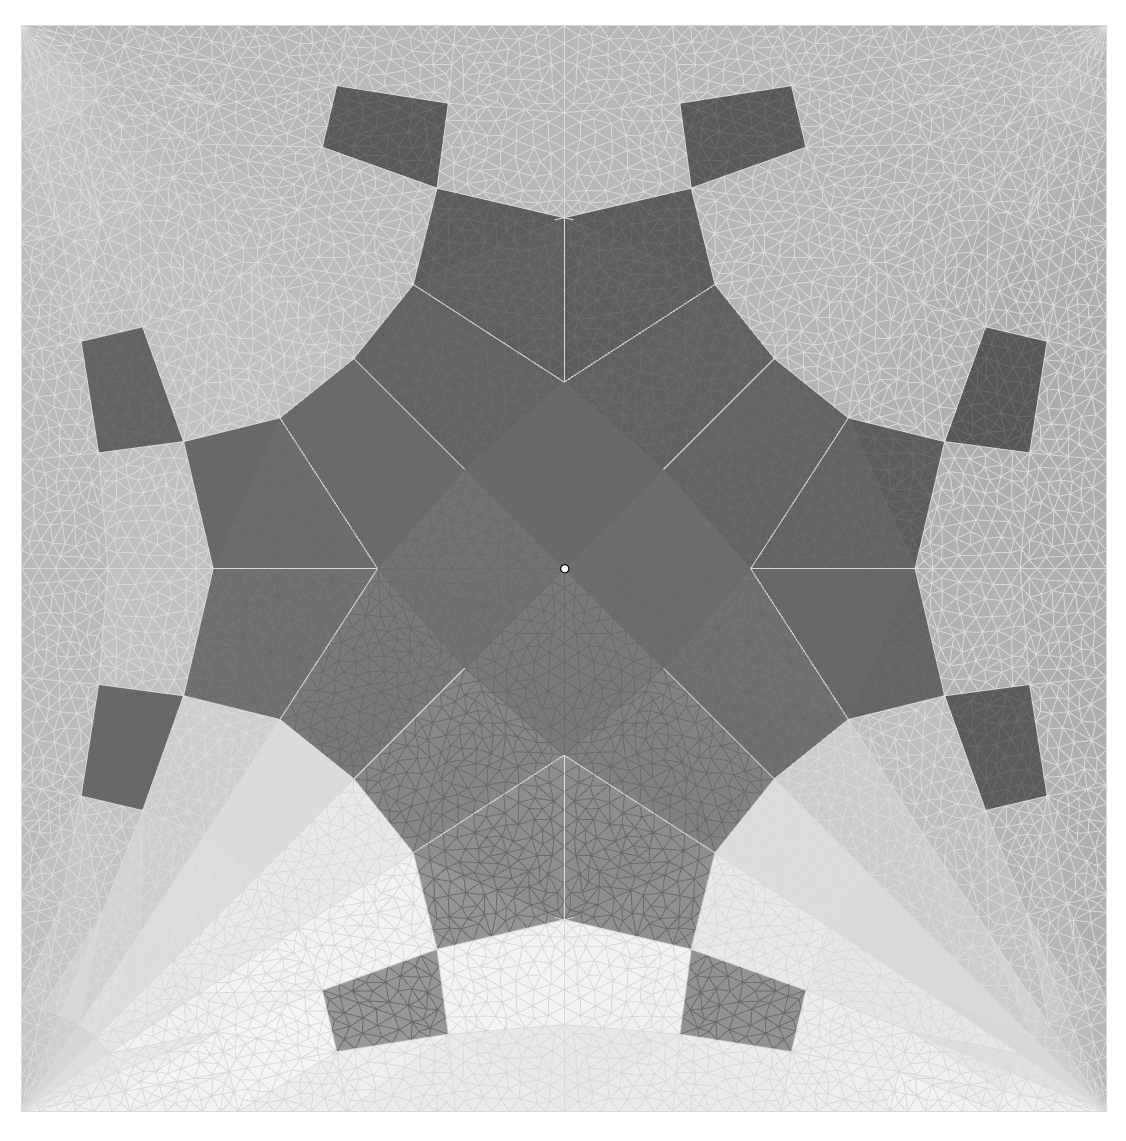
\includegraphics[width=.99\linewidth]{images/t_opt_l2d10_gamma4}
  \caption{$t_{max}/t_{min}=4$}
\end{subfigure}
~
\begin{subfigure}[b]{.32\textwidth}
  \centering
  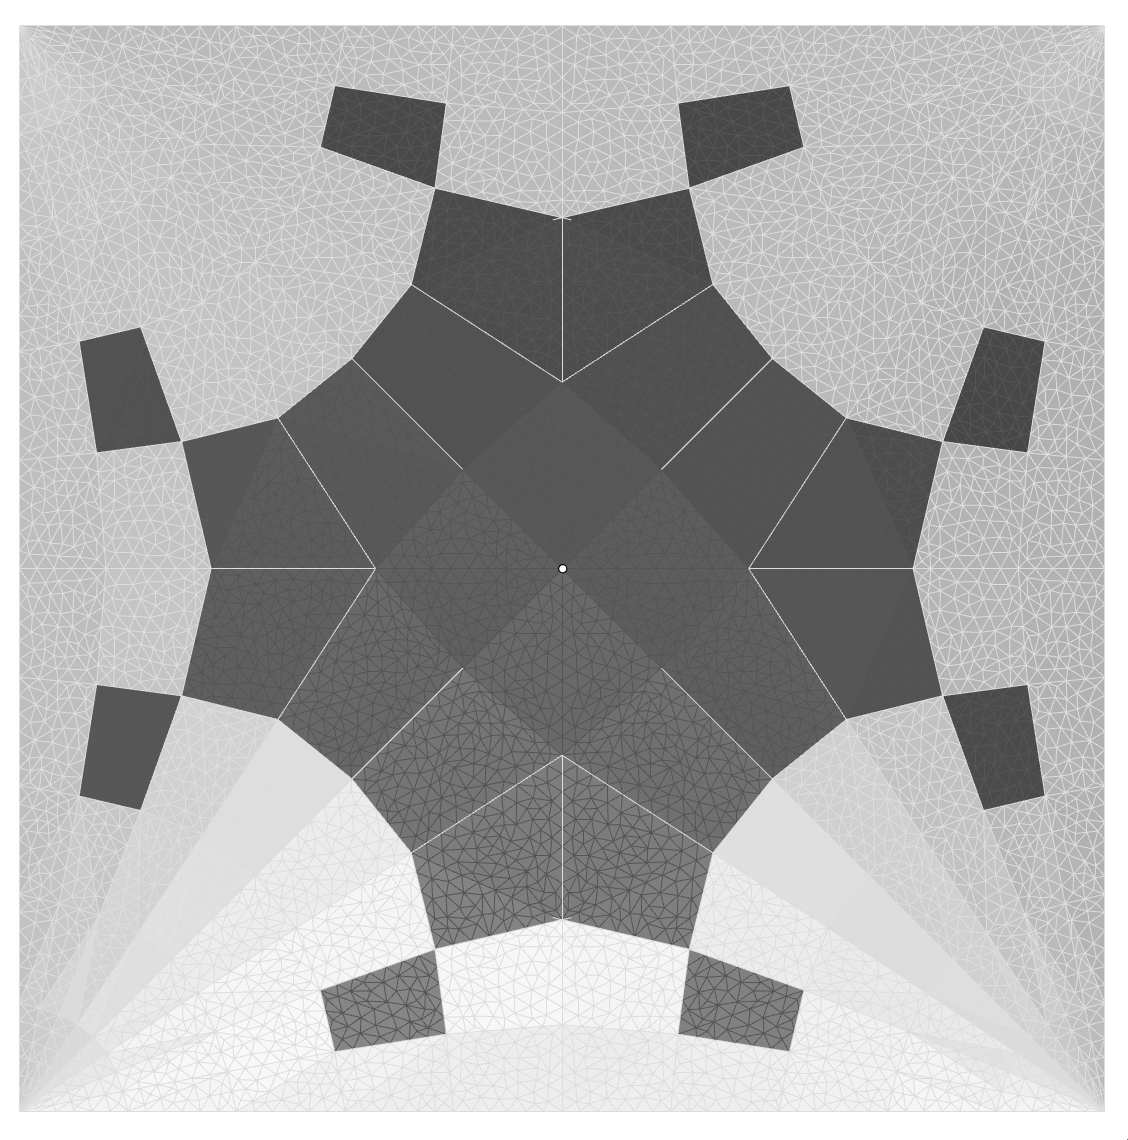
\includegraphics[width=.99\linewidth]{images/t_opt_l2d10_gamma5}
  \caption{$t_{max}/t_{min}=5$}
\end{subfigure}
~
\begin{subfigure}[b]{.32\textwidth}
  \centering
  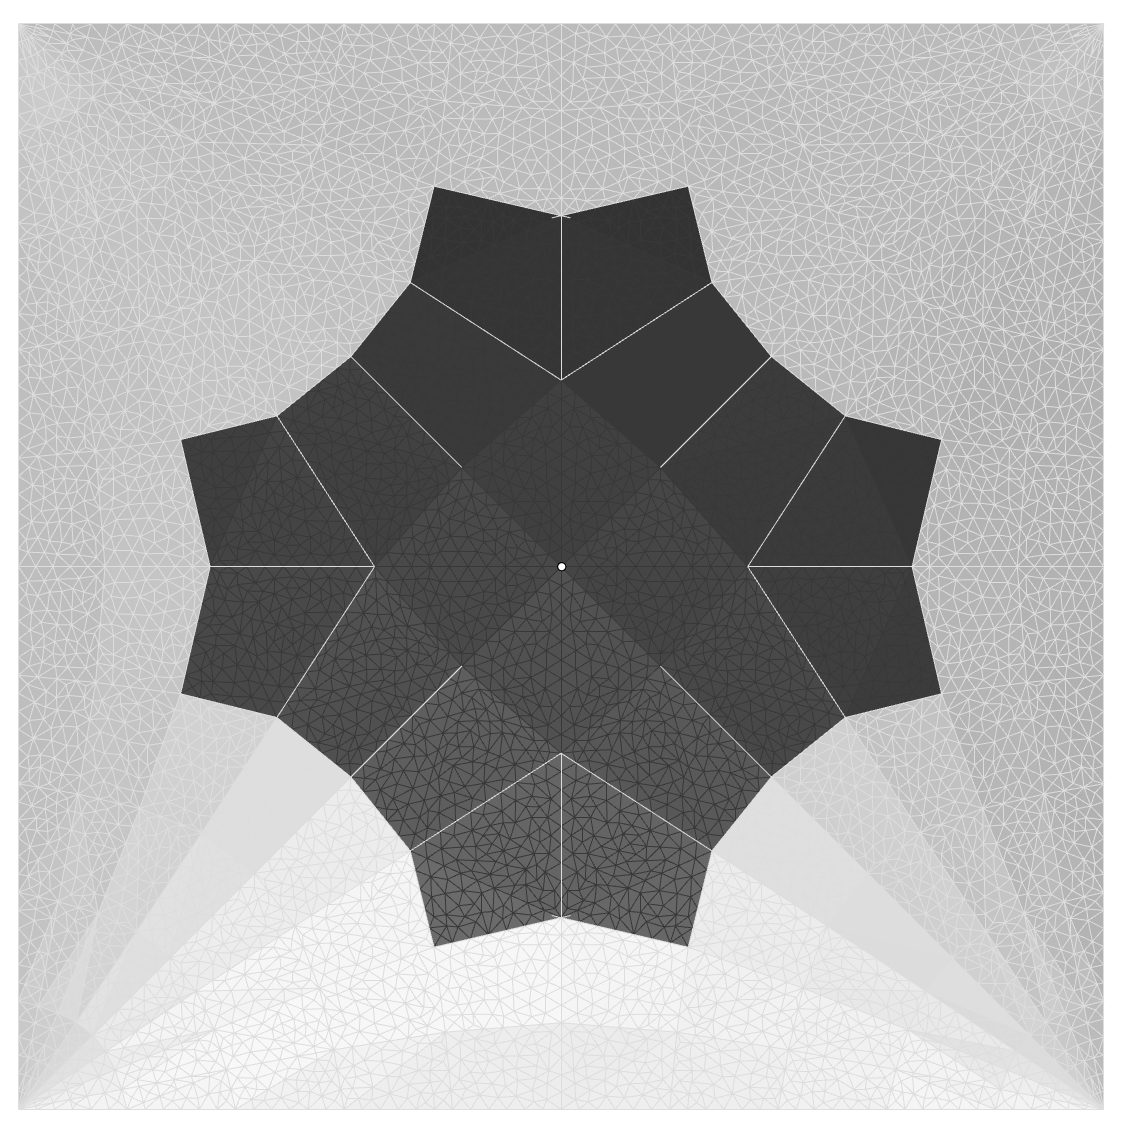
\includegraphics[width=.99\linewidth]{images/t_opt_l2d10_gamma6}
  \caption{$t_{max}/t_{min}=6$}
\end{subfigure}

\begin{subfigure}[b]{.32\textwidth}
  \centering
  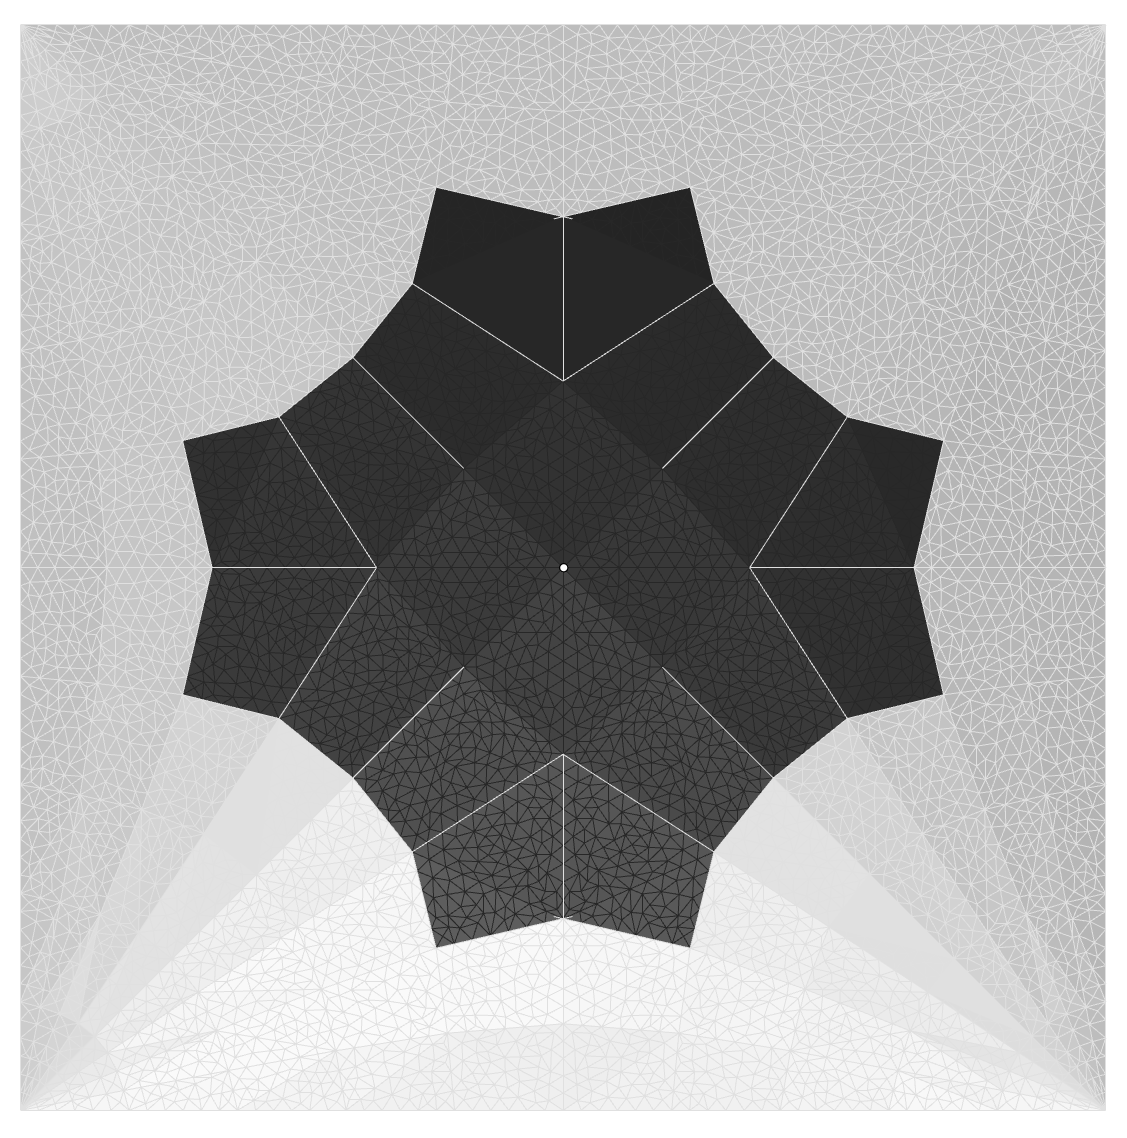
\includegraphics[width=.99\linewidth]{images/t_opt_l2d10_gamma7}
  \caption{$t_{max}/t_{min}=7$}
\end{subfigure}
~
\begin{subfigure}[b]{.32\textwidth}
  \centering
  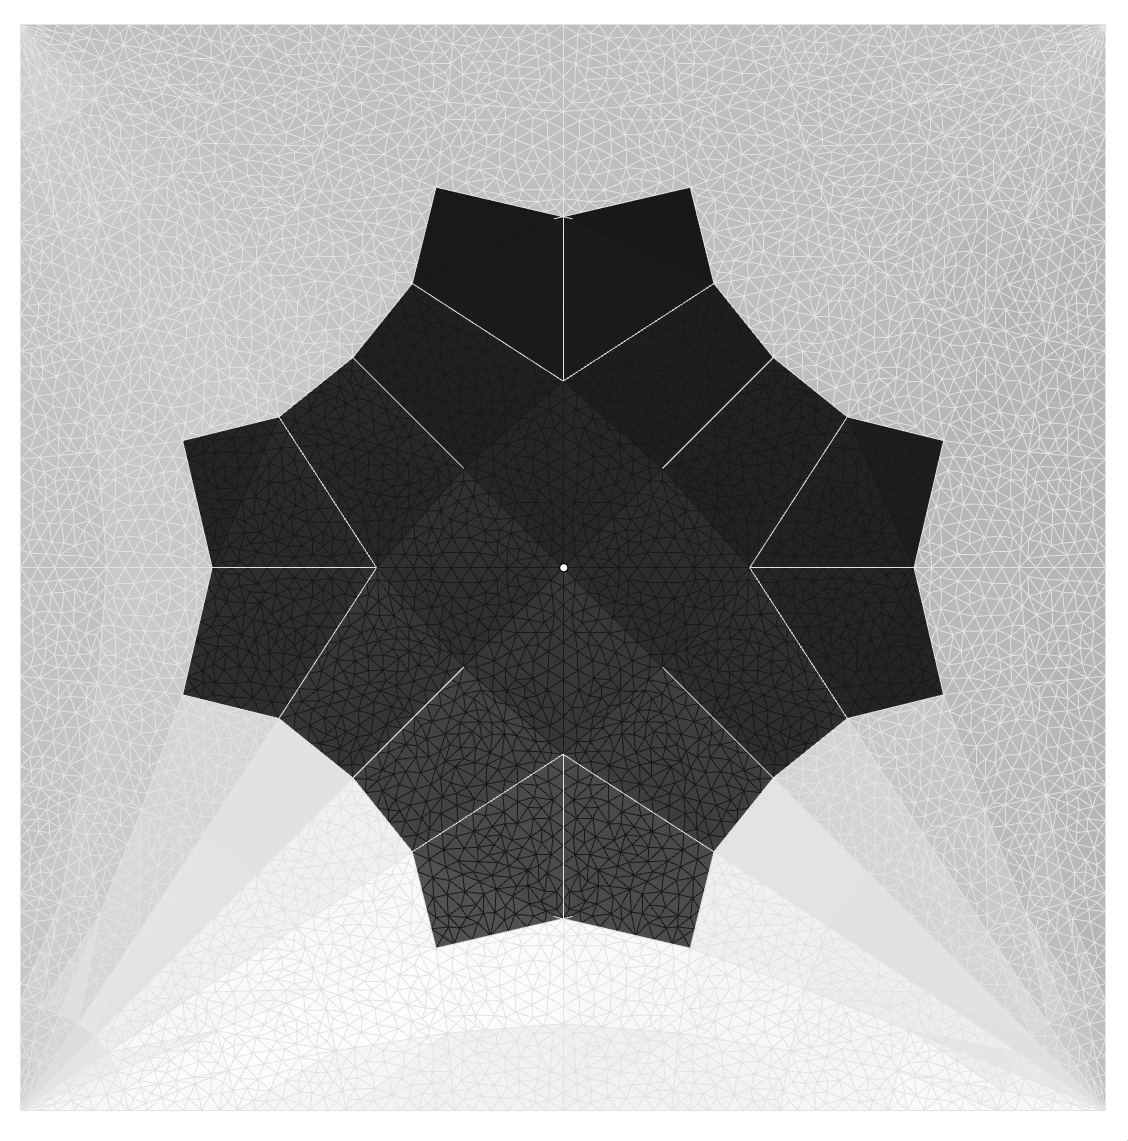
\includegraphics[width=.99\linewidth]{images/t_opt_l2d10_gamma8}
  \caption{$t_{max}/t_{min}=8$}
\end{subfigure}
~
\begin{subfigure}[b]{.32\textwidth}
  \centering
  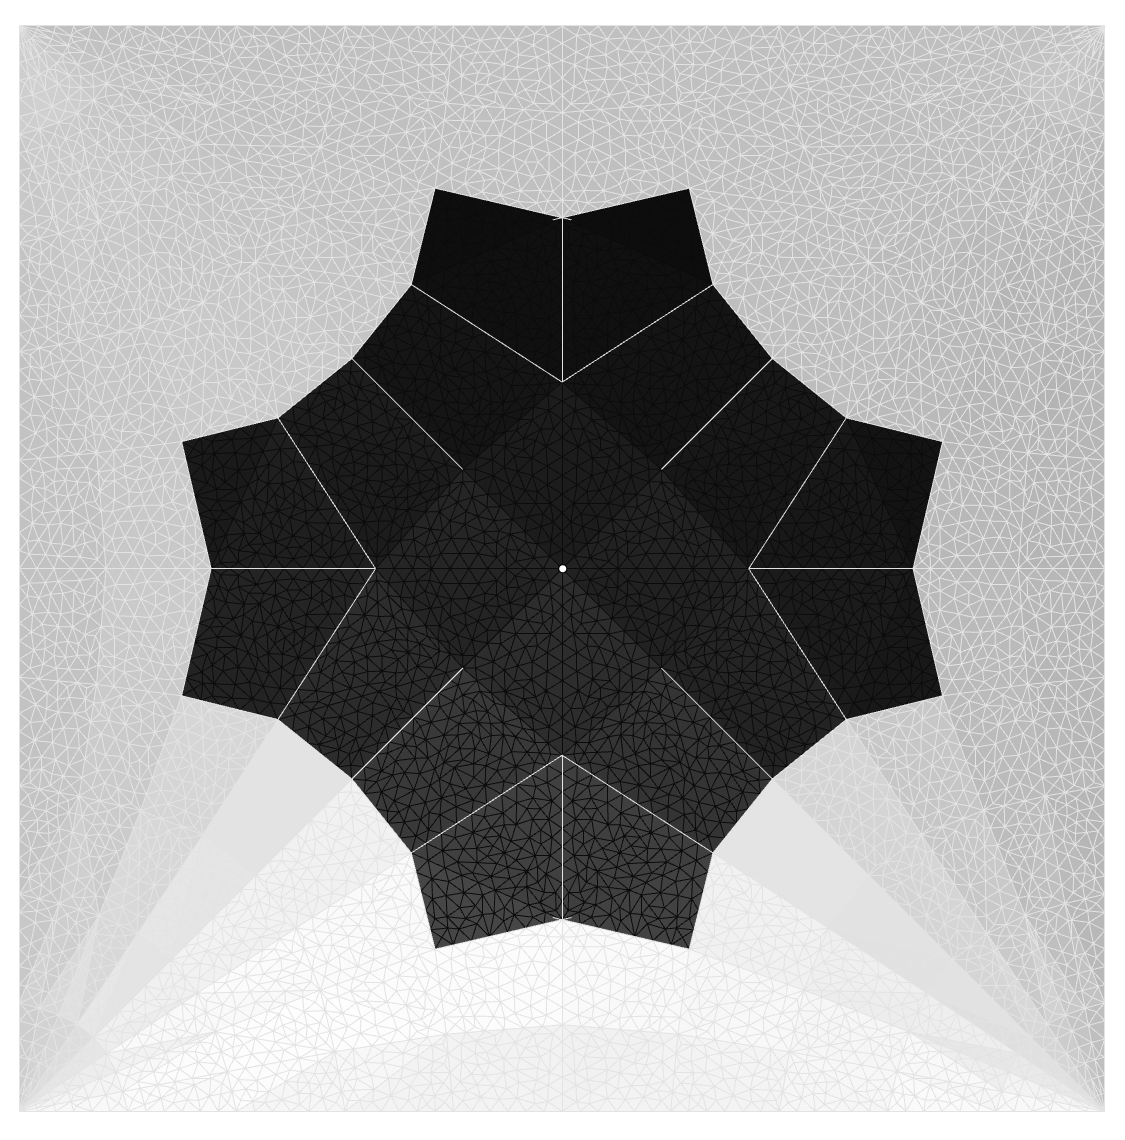
\includegraphics[width=.99\linewidth]{images/t_opt_l2d10_gamma9}
  \caption{$t_{max}/t_{min}=9$}
\end{subfigure}

\begin{subfigure}[b]{.32\textwidth}
  \centering
  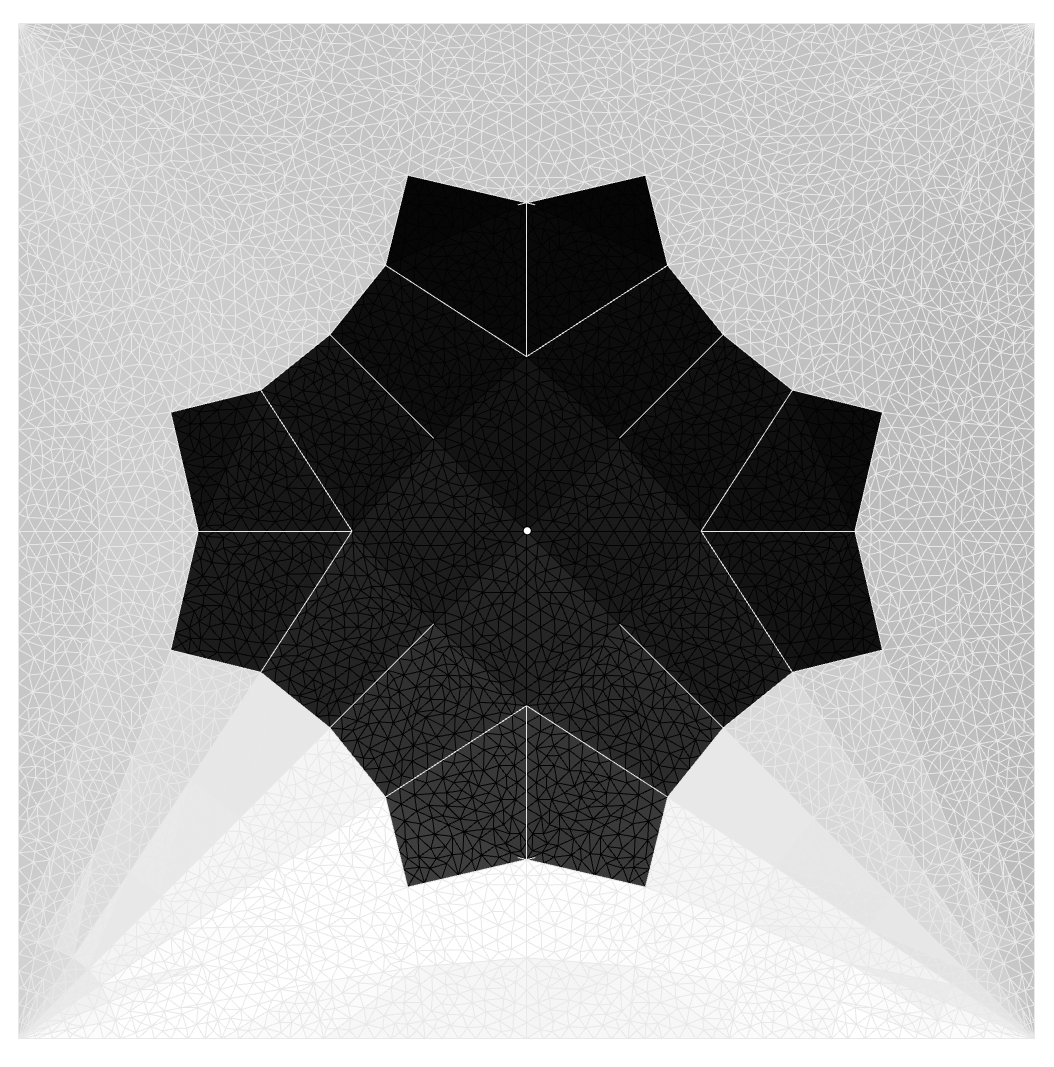
\includegraphics[width=.99\linewidth]{images/t_opt_l2d10_gamma10}
  \caption{$t_{max}/t_{min}=10$}
\end{subfigure}

\caption{Optimized mass distribution of floor $l=5m,l/d=10$}
\label{fig:opt_floor_l2d10}
\end{figure}


\begin{figure}[H]
\begin{subfigure}[b]{.32\textwidth}
  \centering
  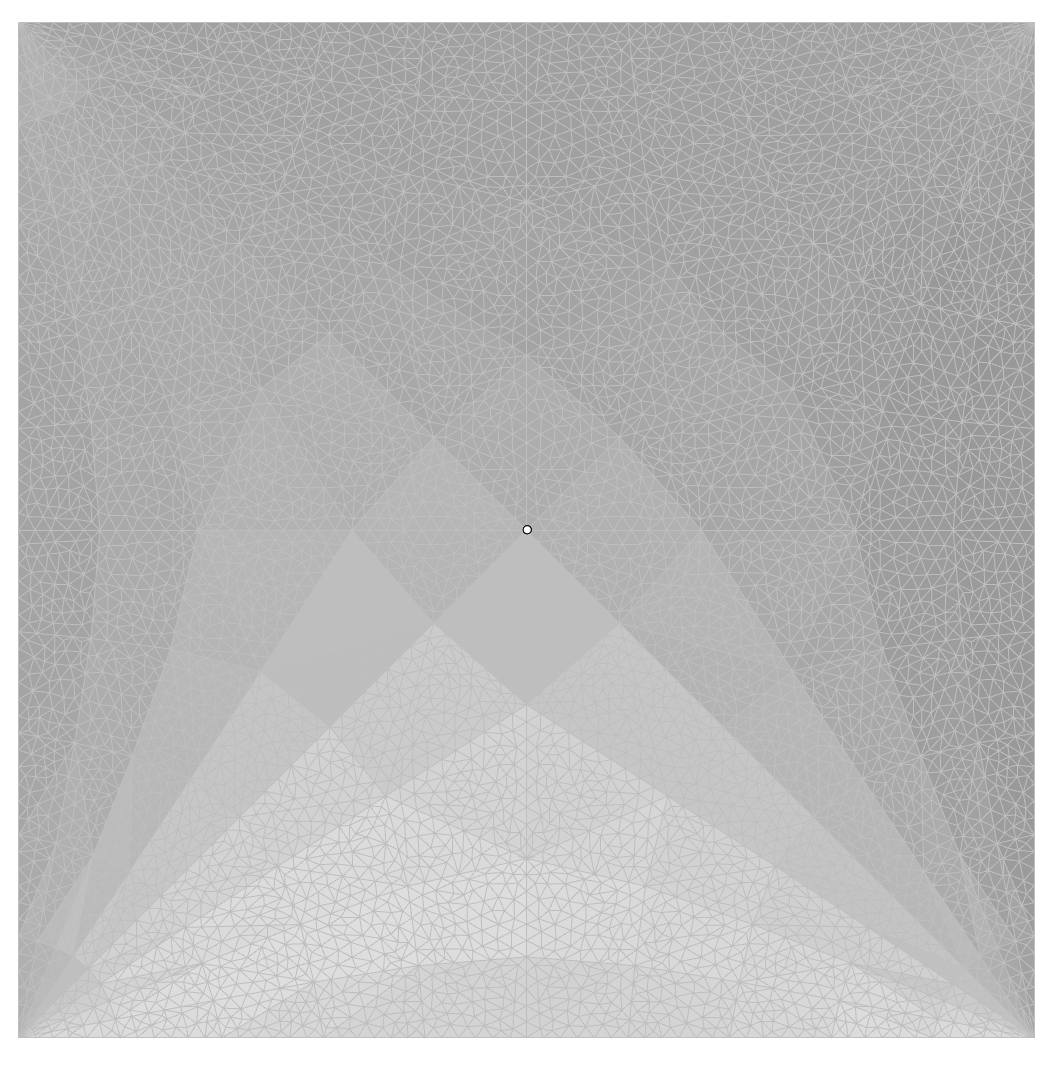
\includegraphics[width=.99\linewidth]{images/t_opt_l2d15_gamma1}
  \caption{$t_{max}/t_{min}=1$}
\end{subfigure}
~
\begin{subfigure}[b]{.32\textwidth}
  \centering
  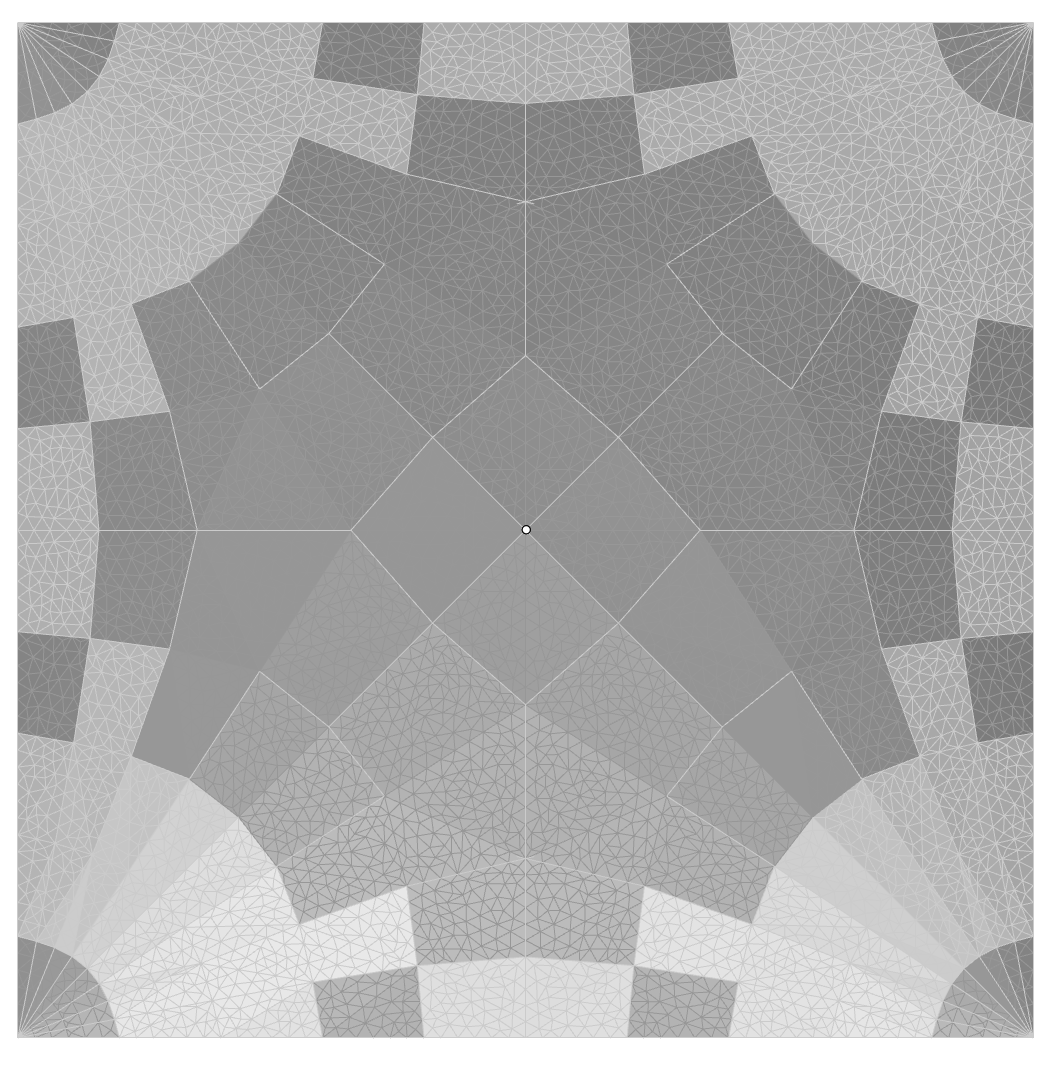
\includegraphics[width=.99\linewidth]{images/t_opt_l2d15_gamma2}
  \caption{$t_{max}/t_{min}=2$}
\end{subfigure}
~
\begin{subfigure}[b]{.32\textwidth}
  \centering
  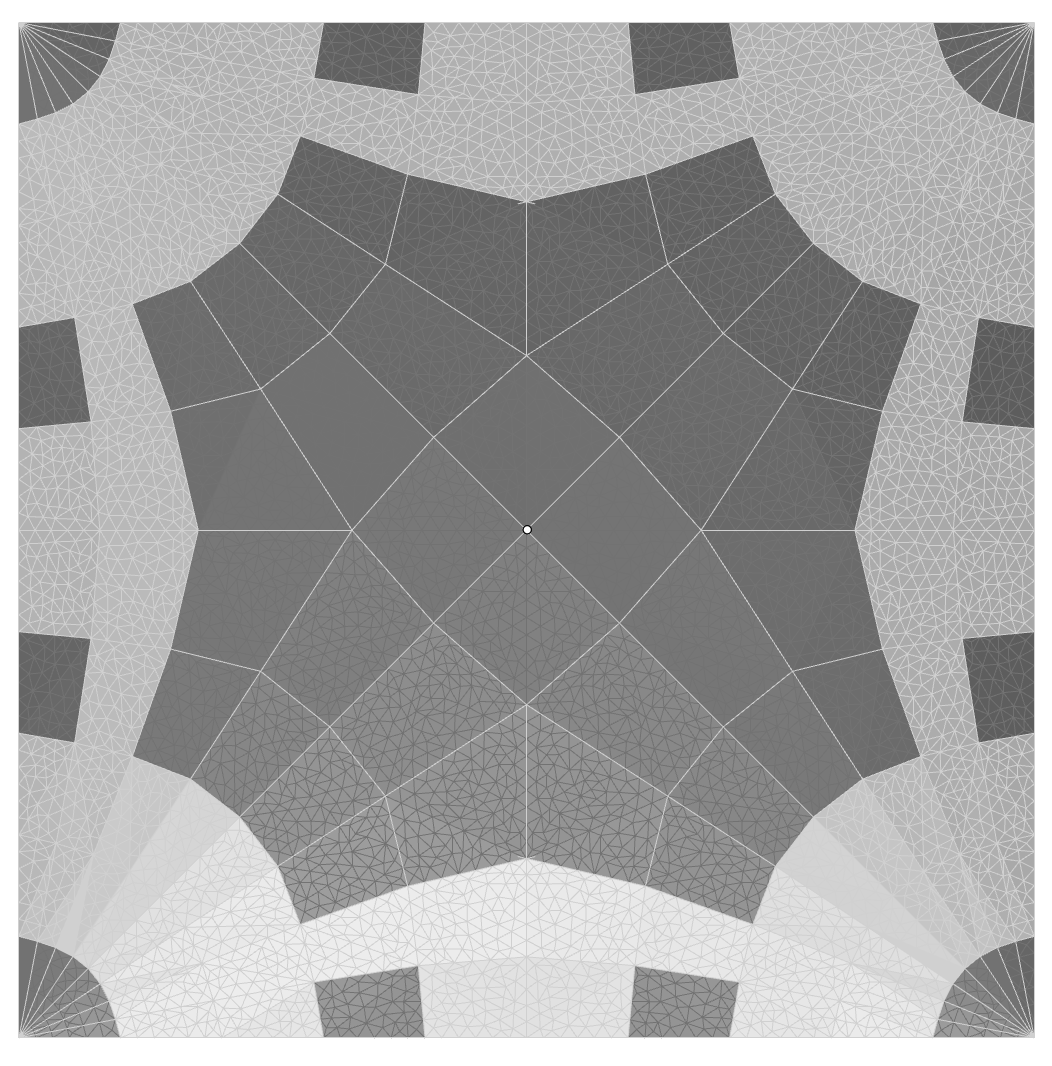
\includegraphics[width=.99\linewidth]{images/t_opt_l2d15_gamma3}
  \caption{$t_{max}/t_{min}=3$}
\end{subfigure}

\begin{subfigure}[b]{.32\textwidth}
  \centering
  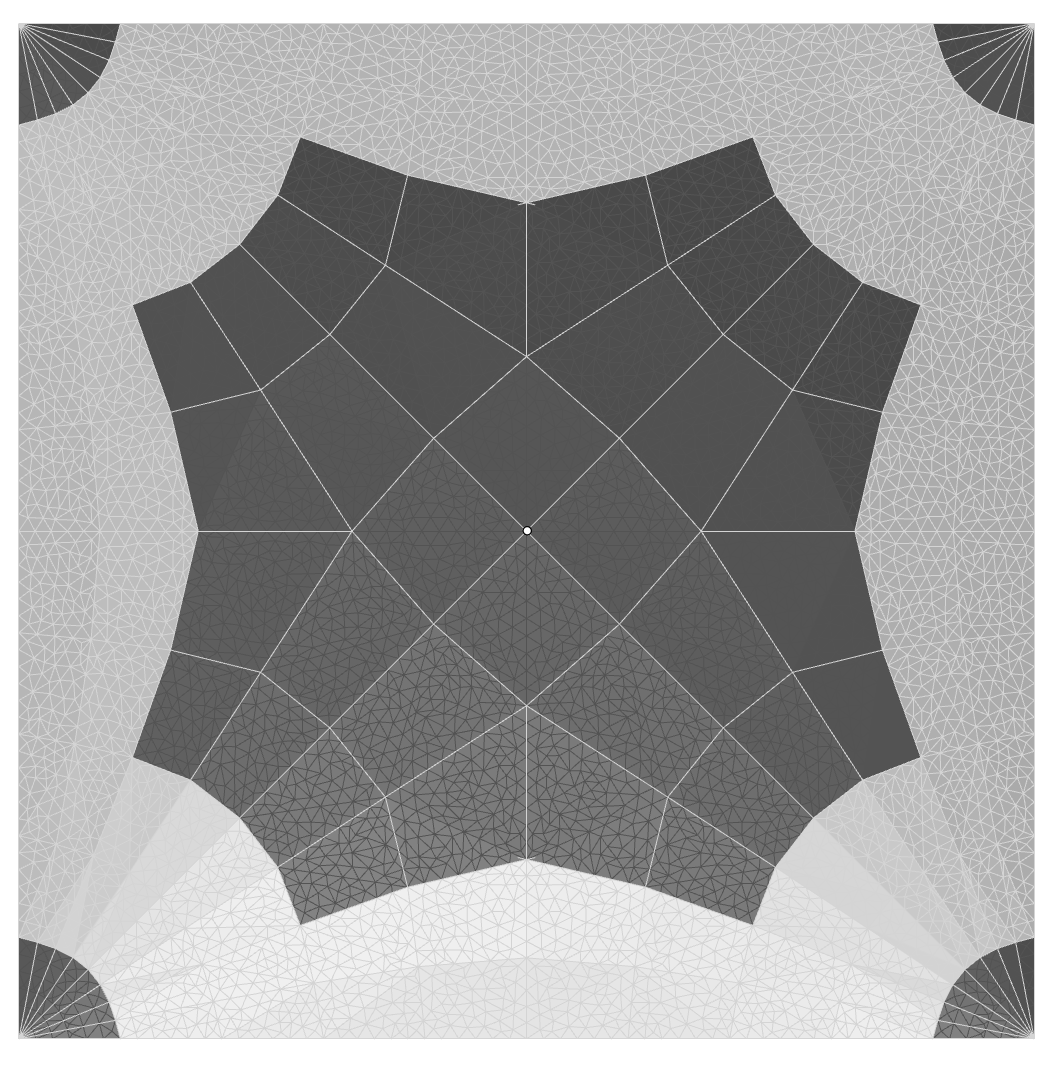
\includegraphics[width=.99\linewidth]{images/t_opt_l2d15_gamma4}
  \caption{$t_{max}/t_{min}=4$}
\end{subfigure}
~
\begin{subfigure}[b]{.32\textwidth}
  \centering
  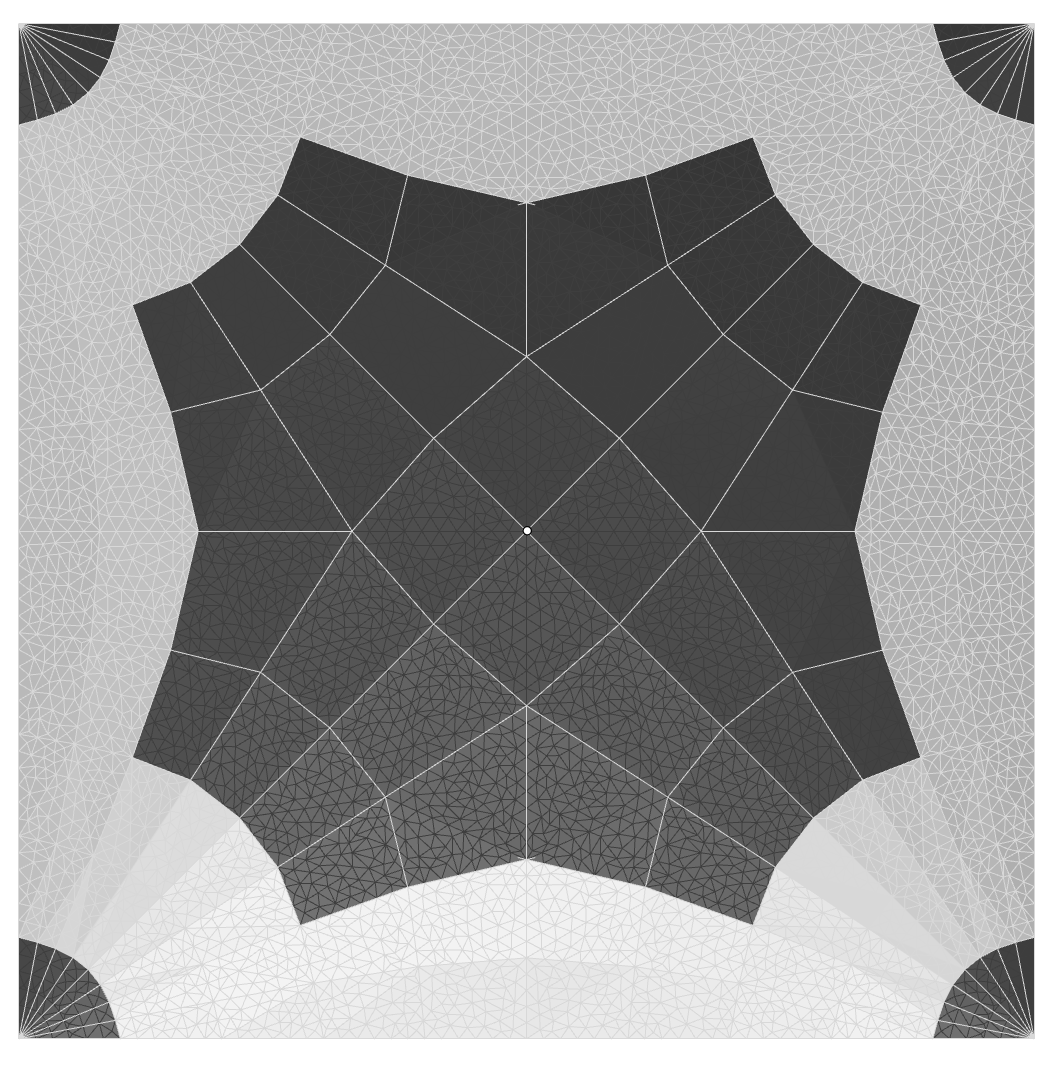
\includegraphics[width=.99\linewidth]{images/t_opt_l2d15_gamma5}
  \caption{$t_{max}/t_{min}=5$}
\end{subfigure}
~
\begin{subfigure}[b]{.32\textwidth}
  \centering
  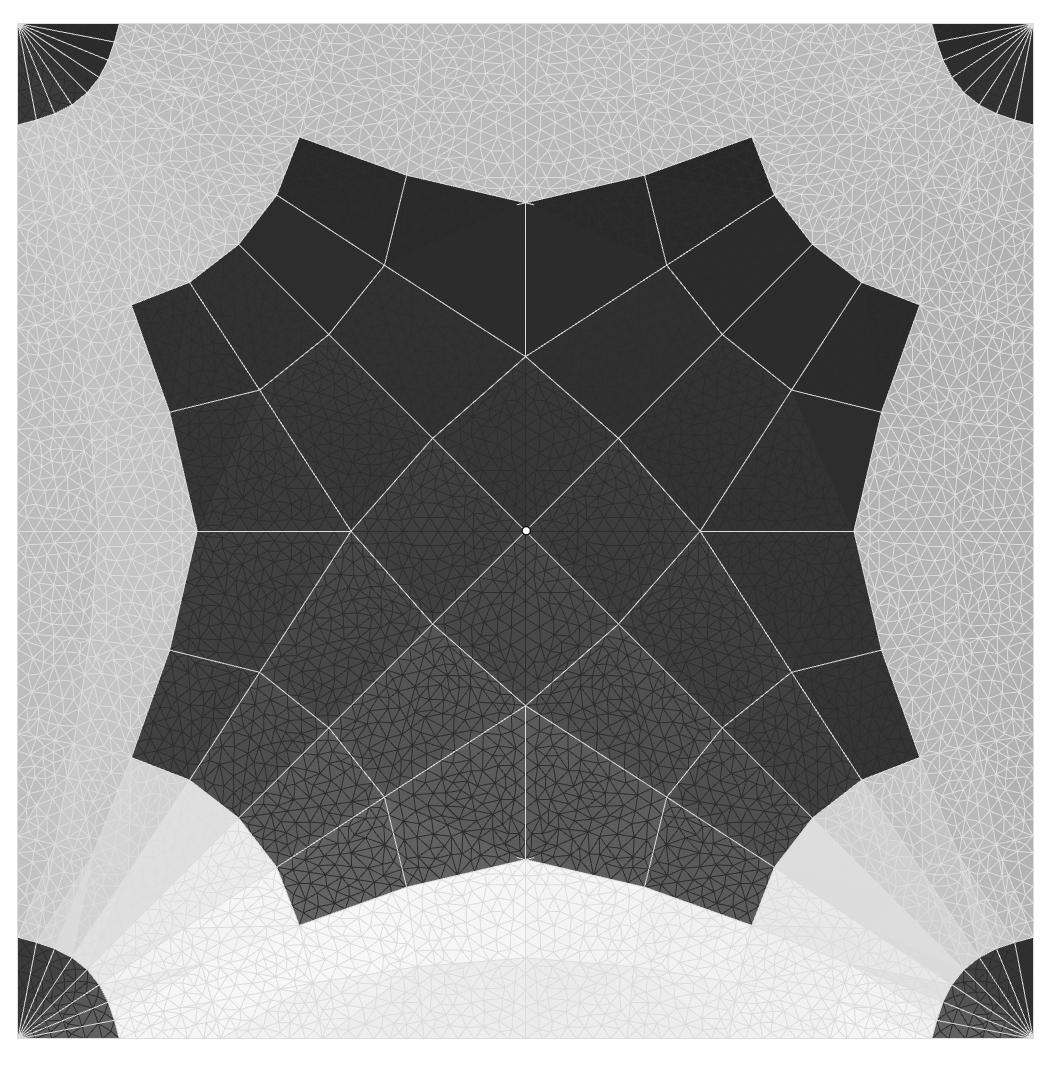
\includegraphics[width=.99\linewidth]{images/t_opt_l2d15_gamma6}
  \caption{$t_{max}/t_{min}=6$}
\end{subfigure}

\begin{subfigure}[b]{.32\textwidth}
  \centering
  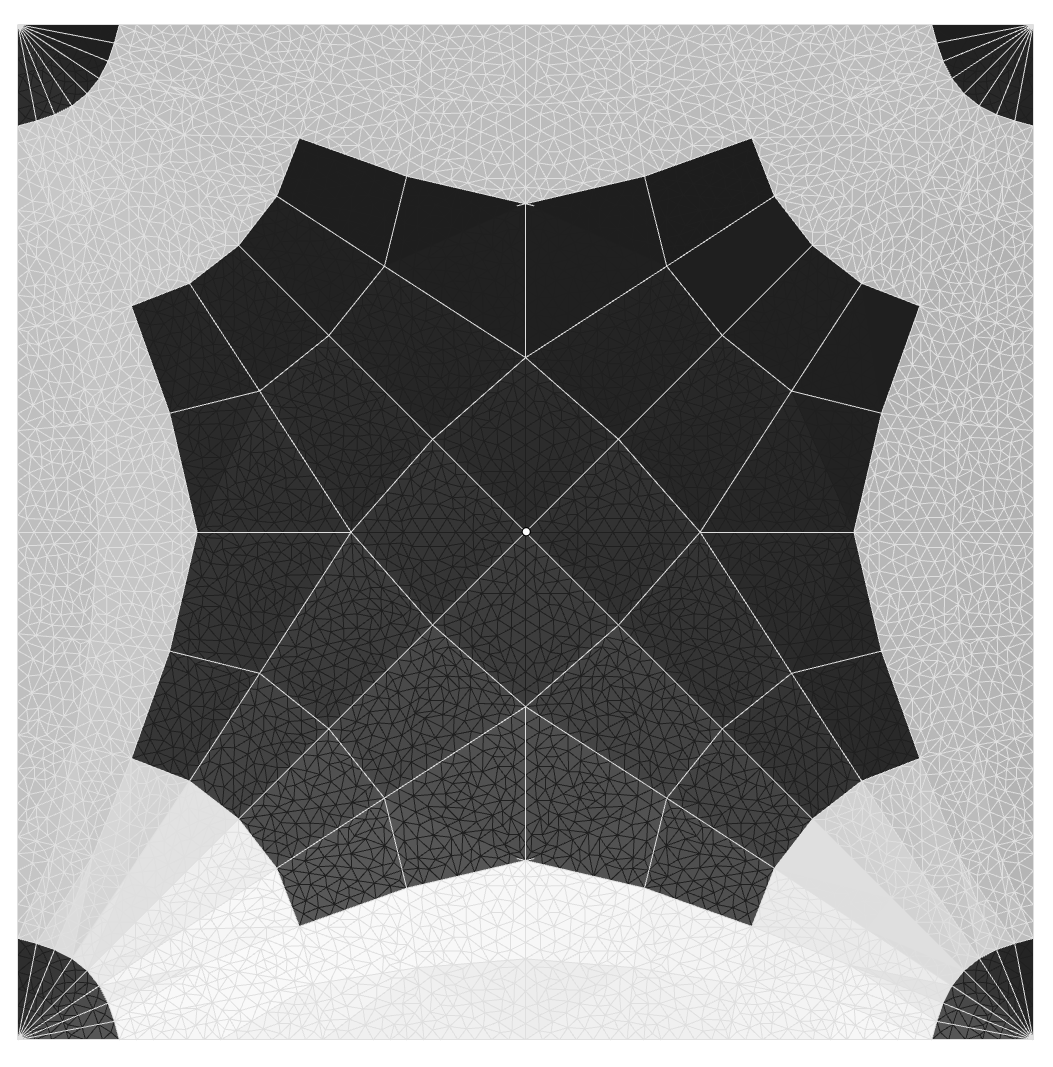
\includegraphics[width=.99\linewidth]{images/t_opt_l2d15_gamma7}
  \caption{$t_{max}/t_{min}=7$}
\end{subfigure}
~
\begin{subfigure}[b]{.32\textwidth}
  \centering
  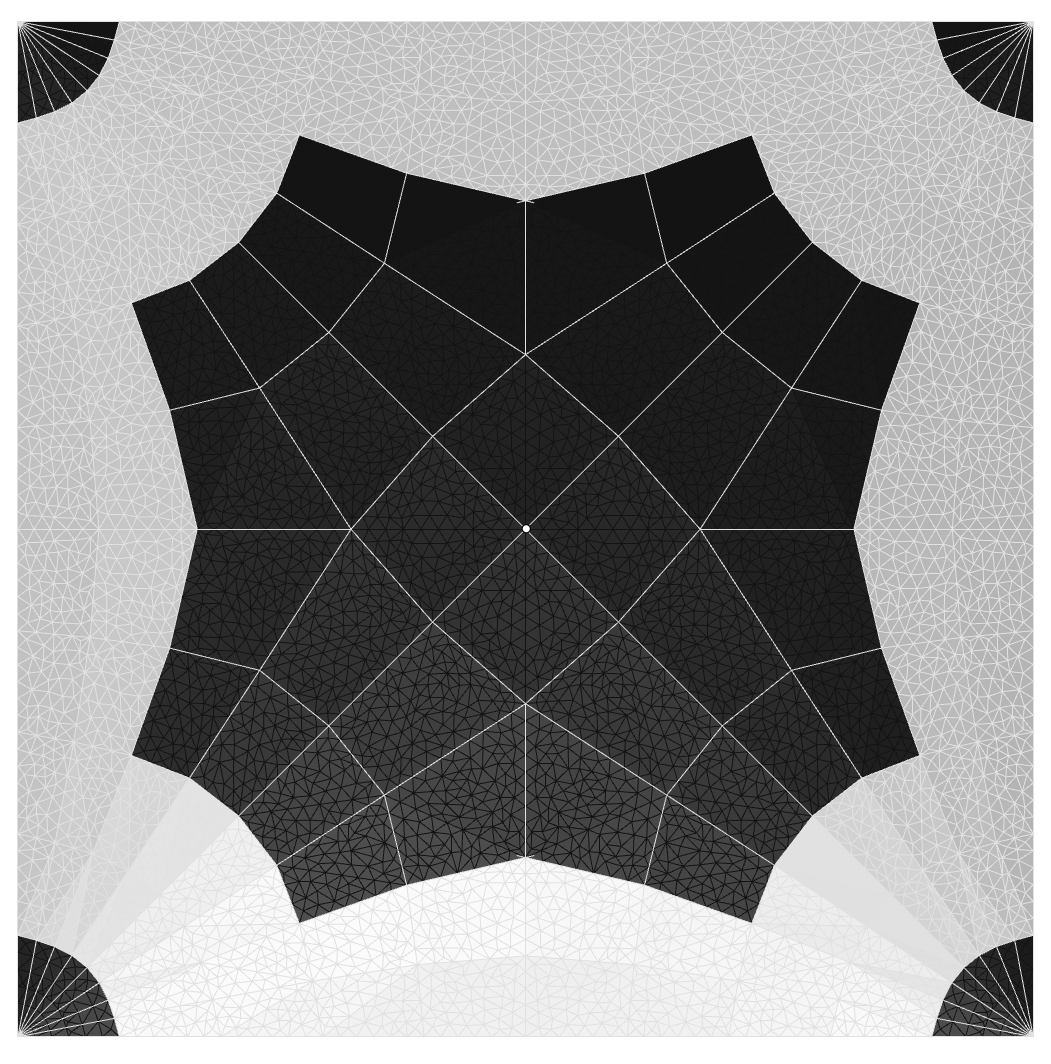
\includegraphics[width=.99\linewidth]{images/t_opt_l2d15_gamma8}
  \caption{$t_{max}/t_{min}=8$}
\end{subfigure}
~
\begin{subfigure}[b]{.32\textwidth}
  \centering
  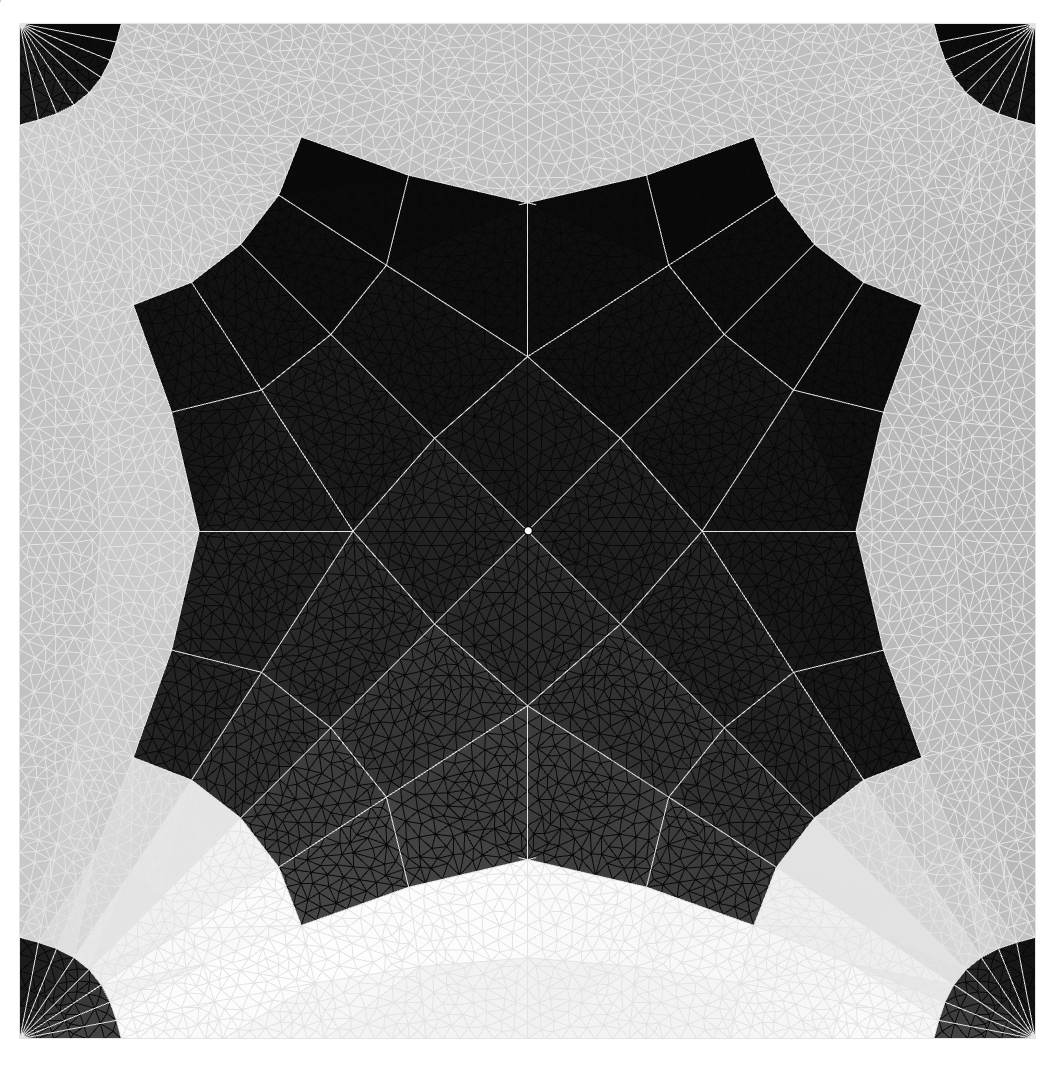
\includegraphics[width=.99\linewidth]{images/t_opt_l2d15_gamma9}
  \caption{$t_{max}/t_{min}=9$}
\end{subfigure}

\begin{subfigure}[b]{.32\textwidth}
  \centering
  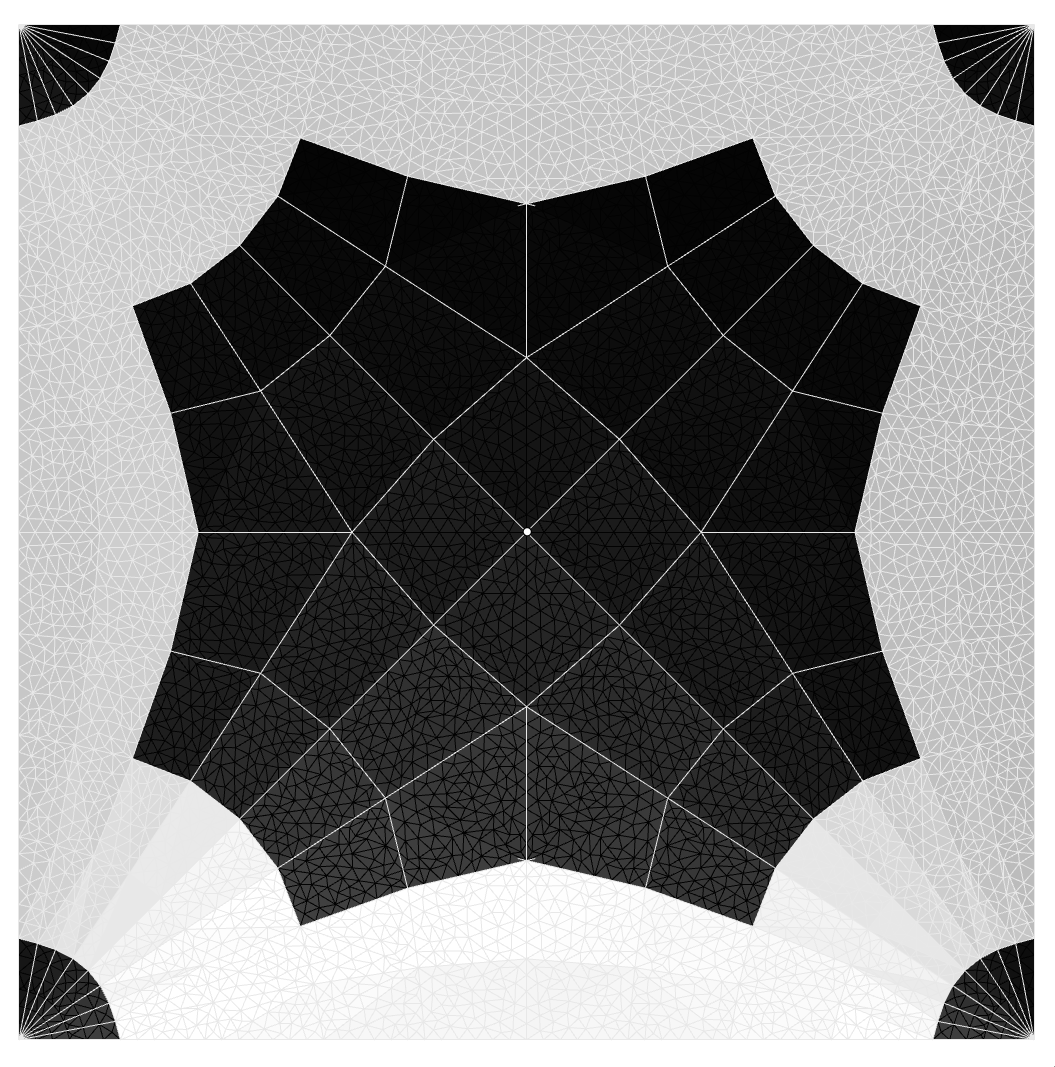
\includegraphics[width=.99\linewidth]{images/t_opt_l2d15_gamma10}
  \caption{$t_{max}/t_{min}=10$}
\end{subfigure}

\caption{Optimized mass distribution of floor $l=5m,l/d=15$}
\label{fig:opt_floor_l2d15}
\end{figure}

Both PCE based optimized floors tend to have thicker panels in the middle and less material in the outer ring, except for the mass concentration on the four supporting edges in figure \ref{fig:opt_floor_l2d15}. The author doubts that such distribution will really benefit the dynamic performance. The optimized mass distribution in figure \ref{fig:opt_floor_l2d10} probably makes more sense, the darker area when $t_{max}/t_{min}\geq 6$ is exactly the region middle 2 in figure \ref{fig:middle_1_2} in pursuit of a higher modal mass while controlling the drop of the natural frequency. Almost the same result was also obtained by Dr. Liew Andrew with pure GA maximizing the modal mass. There the optimized figure was found with the thickness bound [0.01,0.06]m, namely the allowable thickness ratio is 6. The difference is that, the optimization by Dr. Liew was based on a very coarse mesh. Figure \ref{fig:comp_opt} compares the the two optimized results. They represent very similar optimized mass distribution, except for some small differences in the ribs.

\begin{figure}[H]
\begin{subfigure}[c]{.49\textwidth}
  \centering
  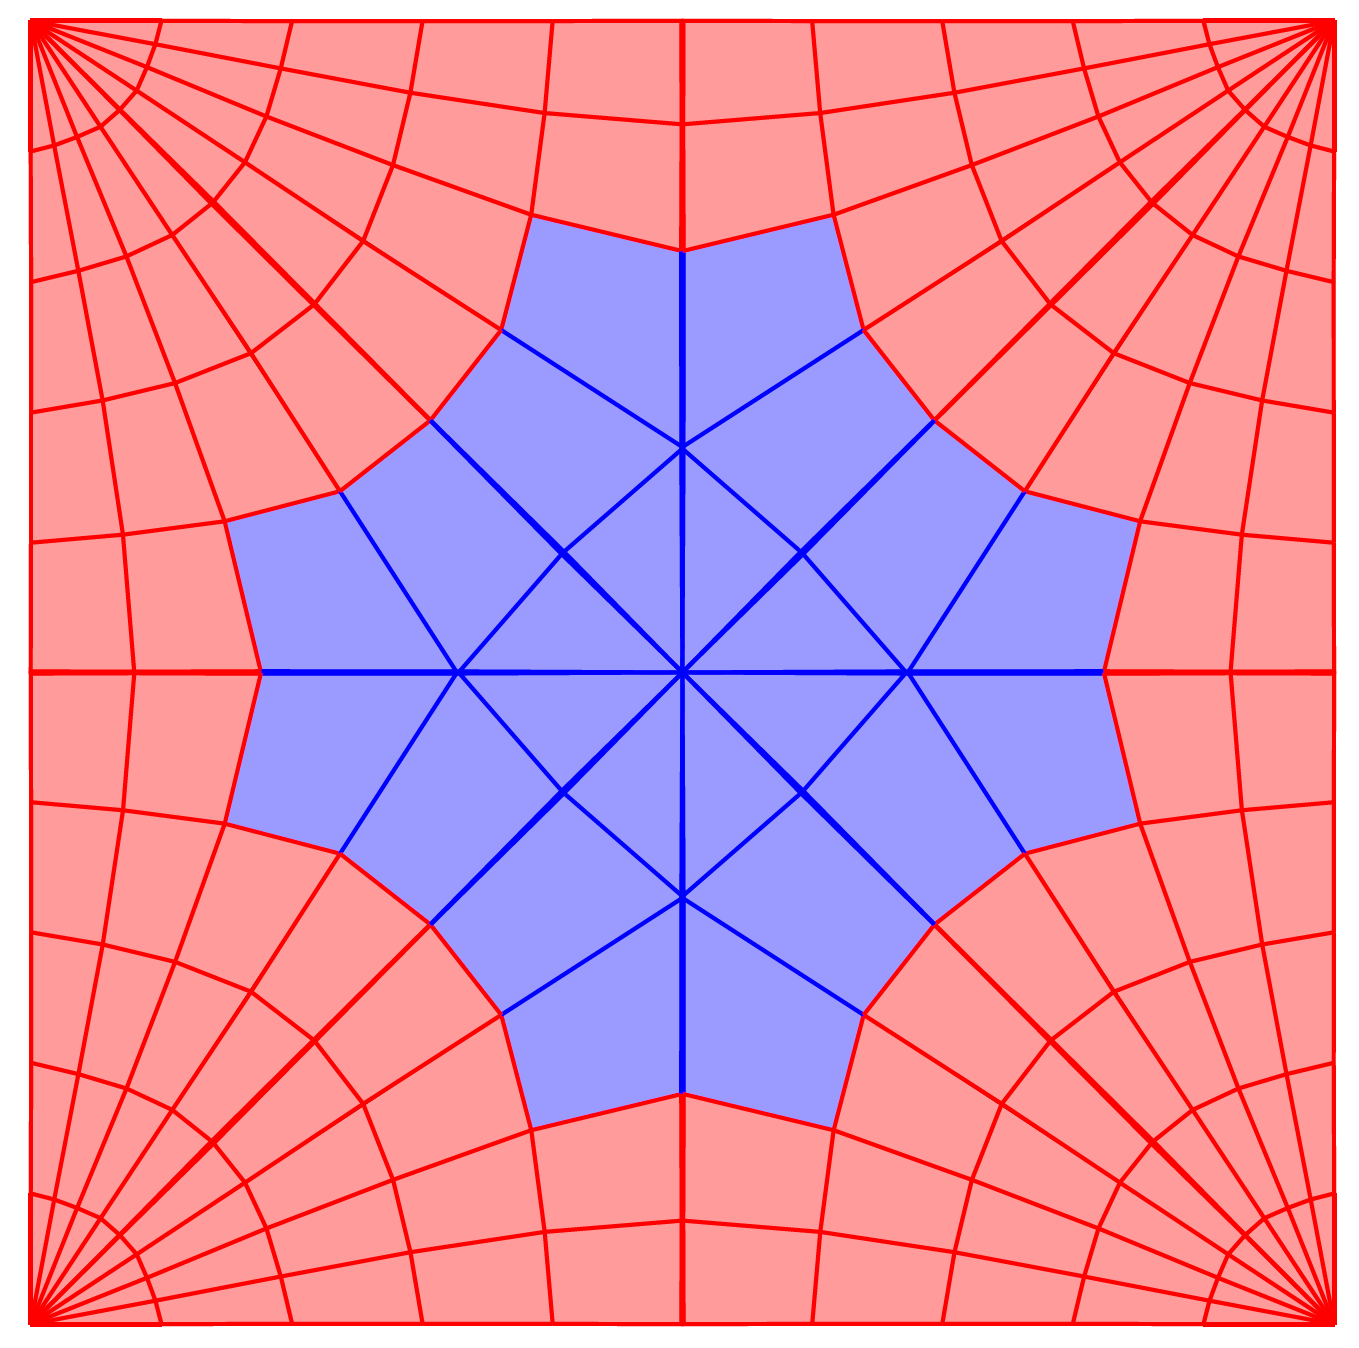
\includegraphics[width=.99\linewidth]{images/opt_m1}
  \caption{Pure GA, maximizing $m_1$ (blue=thick, red=thin)}
\end{subfigure}
~
\begin{subfigure}[c]{.49\textwidth}
  \centering
  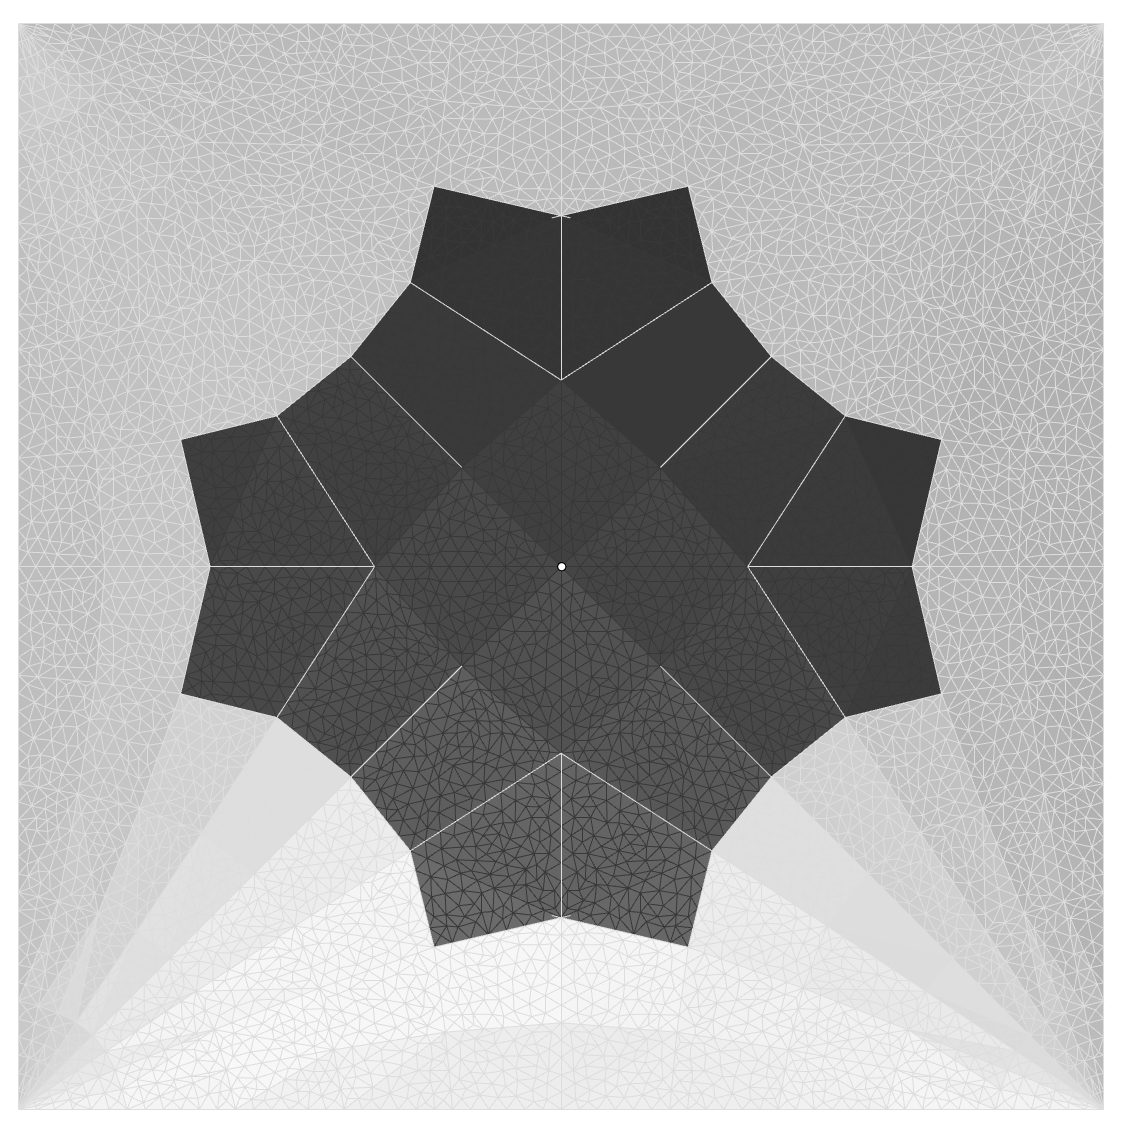
\includegraphics[width=.985\linewidth]{images/t_opt_l2d10_gamma6}
  \caption{PCE based GA, minimizing $R_1$, $t_{max}/t_{min}$=6}
\end{subfigure}

\caption{Mass distribution of two optimized floors with different schemes}
\label{fig:comp_opt}
\end{figure}
 
The two PCE models, one is built on not very smart input samples, but leads to relatively more reasonable results. This indicates a deficiency in its robustness. To optimize a model with 41 dimensions through 84 evaluations of full model is difficult. However, both models show a similar trend in redistributing the mass. The improvements of their dynamic performance compared to the initial floors with uniform thickness in vault and ribs respectively are illustrated in figure \ref{fig:gamma_R1_opt}. Even though they are not likely to be perfectly optimized, considerable reductions in the response have been achieved. Especially when the high complexity of the model and the low computational effort are considered. Less than 90 min were needed to run the experimental designs and build the PCE model, 50000 evaluations (100 populations, 500 generations) of the PCE model for one GA optimization took only 30s. 

\begin{figure}[H]
\begin{subfigure}[b]{.9\textwidth}
  \centering
  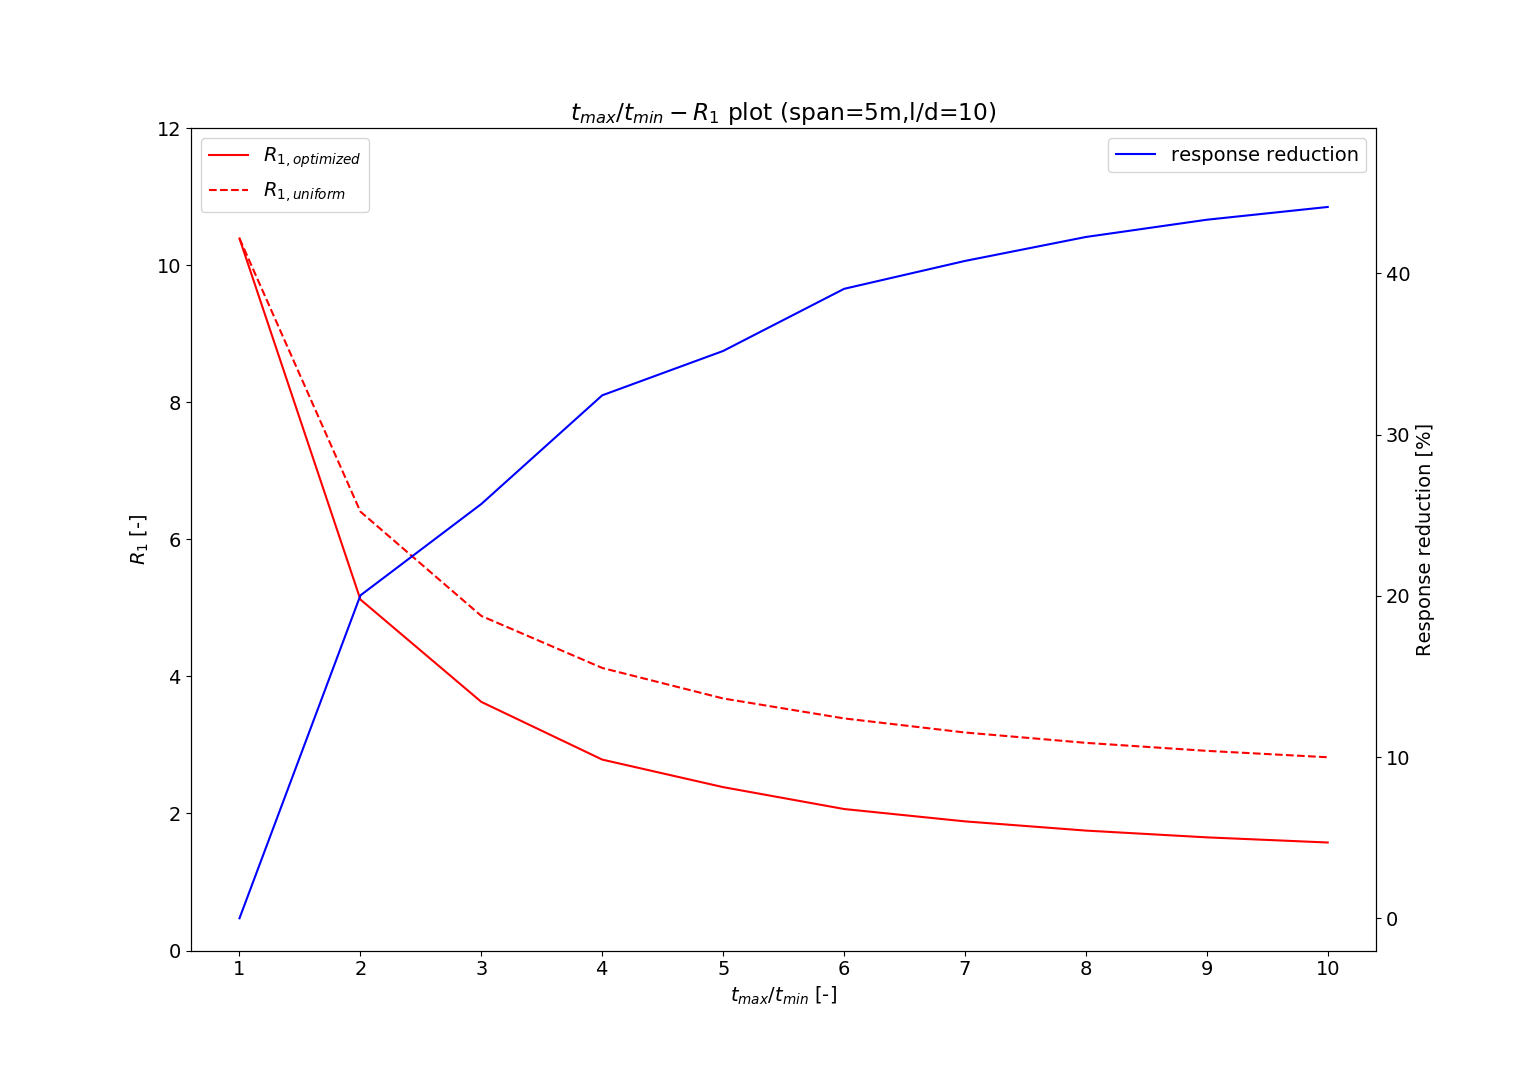
\includegraphics[width=.99\linewidth]{images/gamma_R1_l2d10}
  \caption{Floor l=5m,$l/d=10$}
\end{subfigure}

\begin{subfigure}[b]{.9\textwidth}
  \centering
  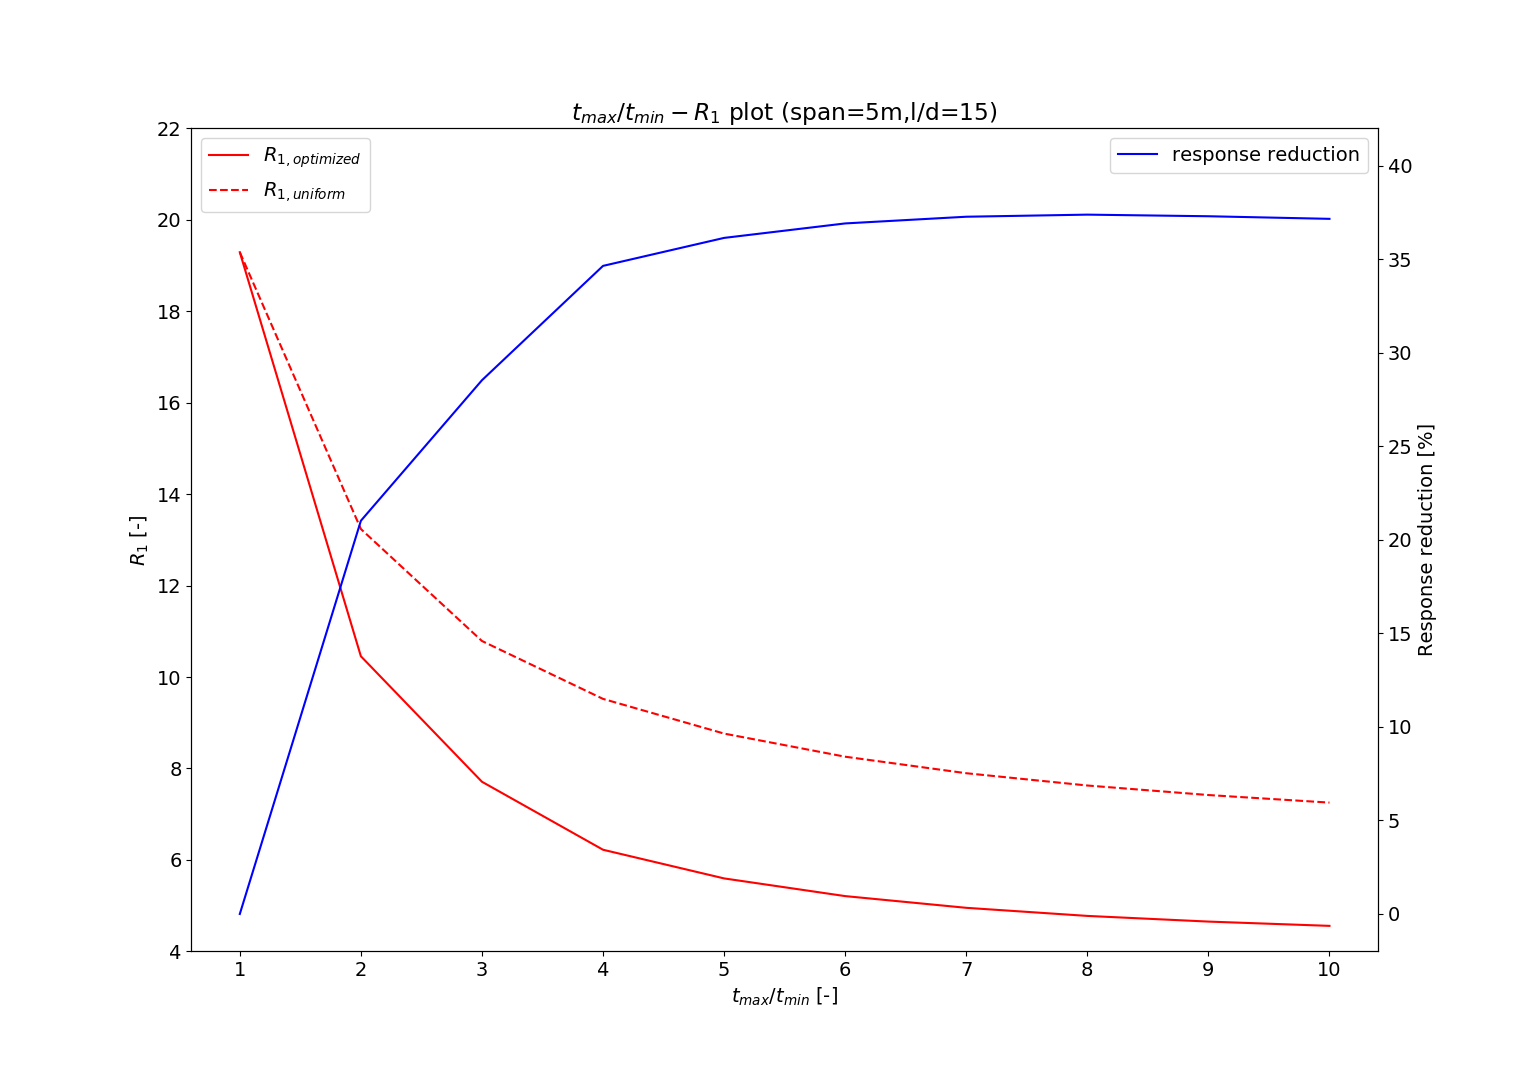
\includegraphics[width=.99\linewidth]{images/gamma_R1_l2d15}
  \caption{Floor l=5m,$l/d=15$}
\end{subfigure}

\caption{Comparison of dynamic performance between initial and optimized floors}
\label{fig:gamma_R1_opt}
\end{figure}

A big advantage such surrogate models can bring along is that, a deep understanding of the mechanism behind is not a must. In many cases, the influential parameters and their relation to the output are not easy to find. With such a machine learning alike process, the surrogate model can learn and recognize the important parameters by itself from the experimental designs. The relative significance of these panels can be easily identified from the coefficients before them in the PCE model.





























